\chapter{Results from the averaging learning on 3 datasets}
\label{app:C}
The figures shown in this appendix serve as a completion on the figures that were presented in the discussion of section \ref{s:averaging_method}. It concerns the results of the learning algorithm that learns from three ideal datasets. Figure C.1 displays the convergence during the learning process and plots $\bm{f}_{rel}$ over the iterations. Figure C.2 shows the absolute difference between the learned and observed features. In Figure C.3 the learning of the weights towards the final ones are presented. Figure C.4 presents the difference of current weight with respect to the previous one and as last Figure C.5 shows which of the three RPROP cases that is used in order to update a certain weight. 

\begin{figure}[h!]\label{stijn}
	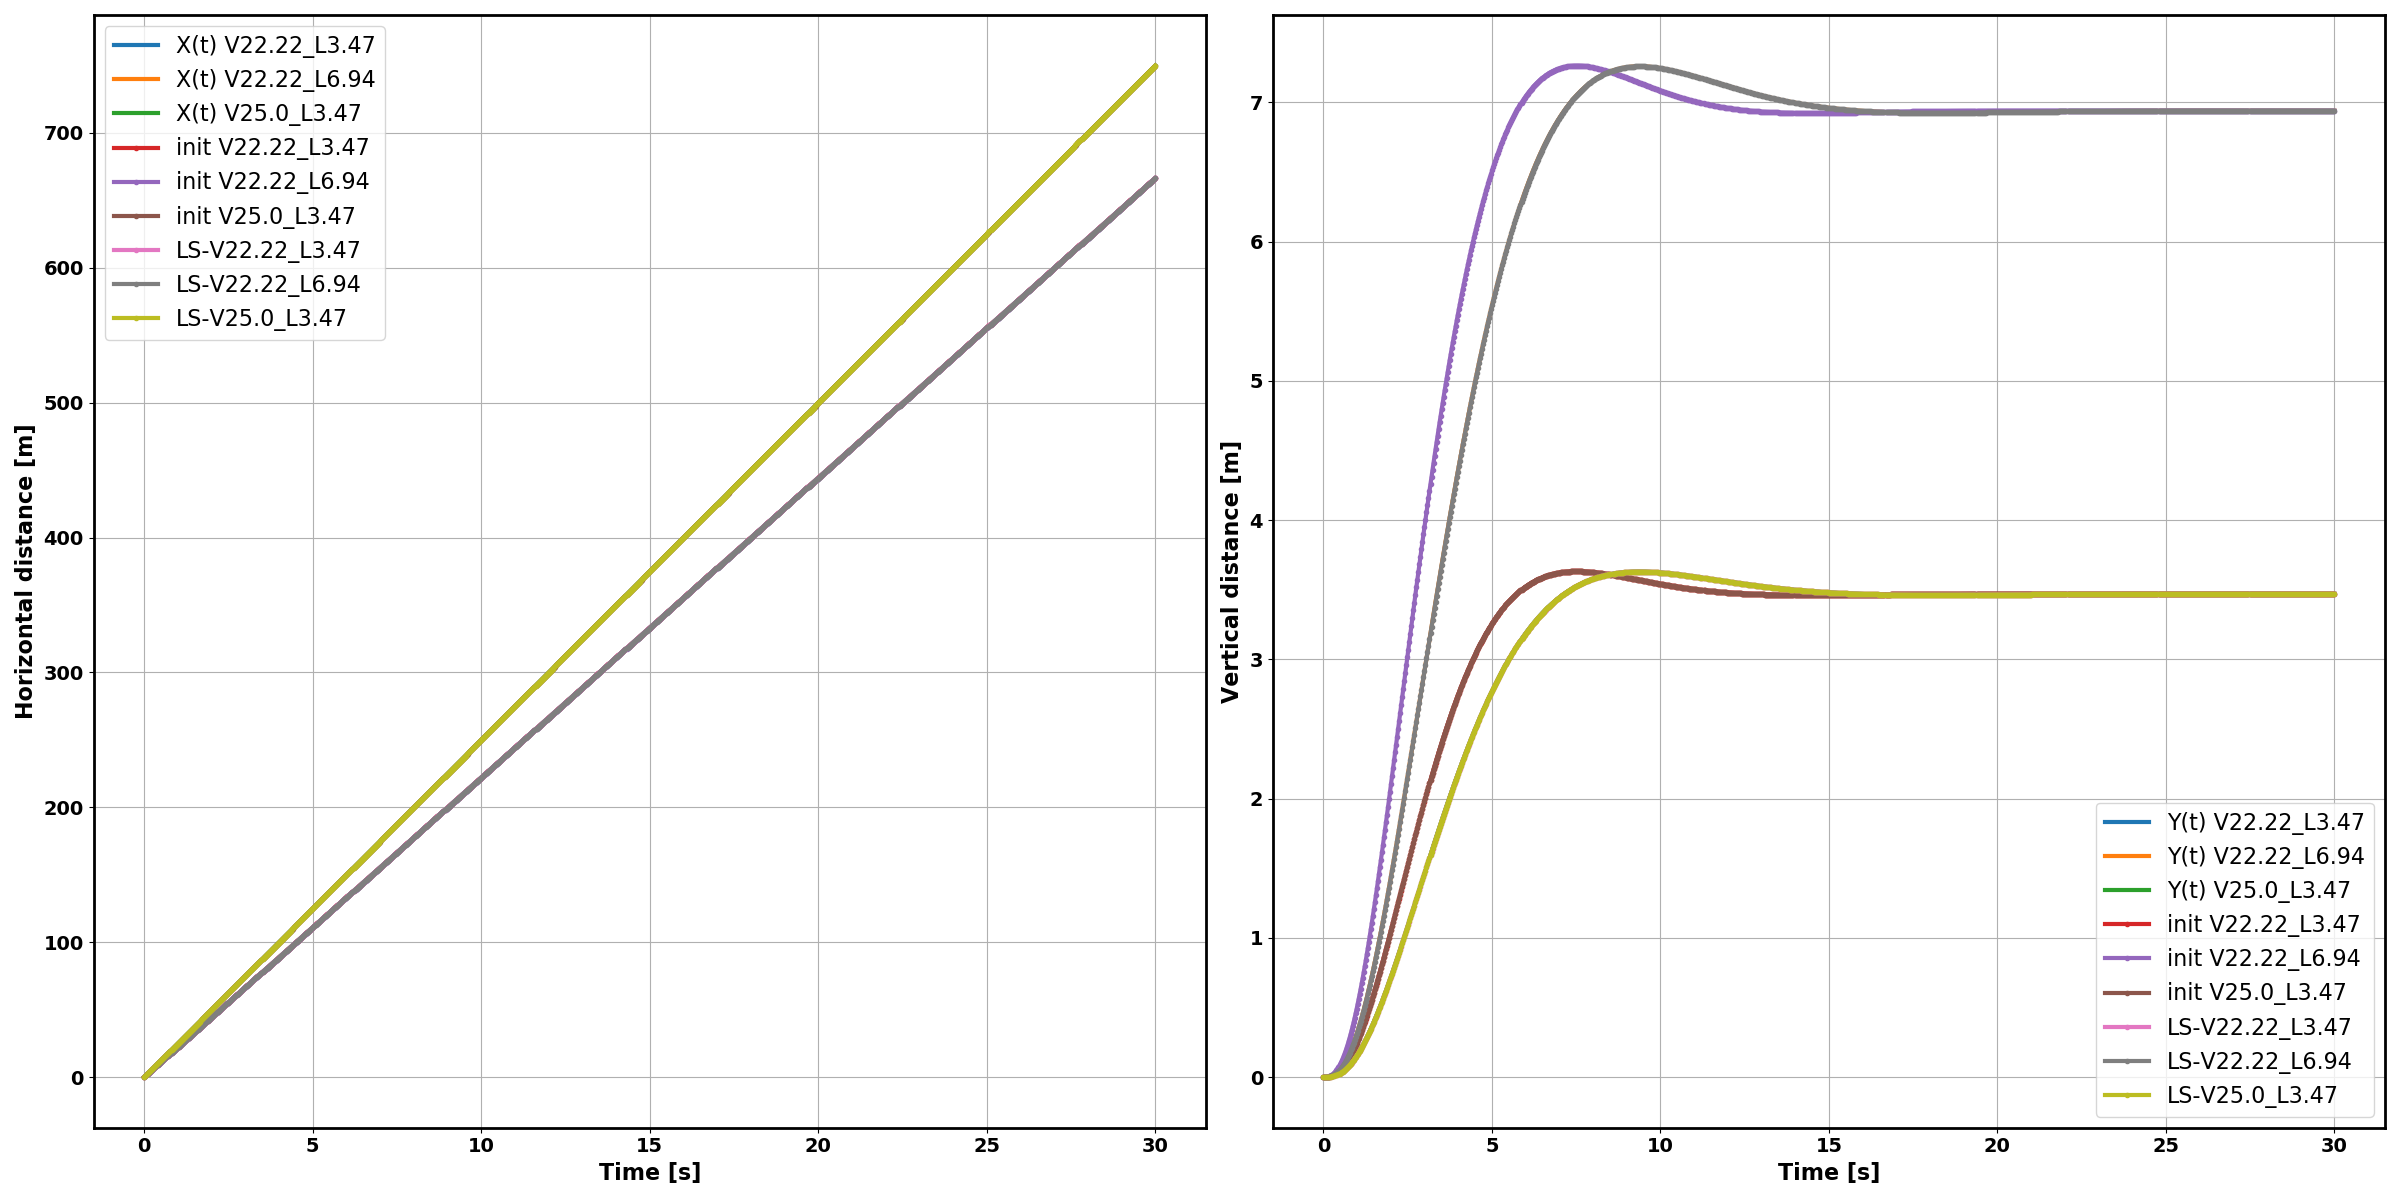
\includegraphics[width=1.0\textwidth]{1l.png}
\end{figure}


\begin{figure}[h!]
	\centering
	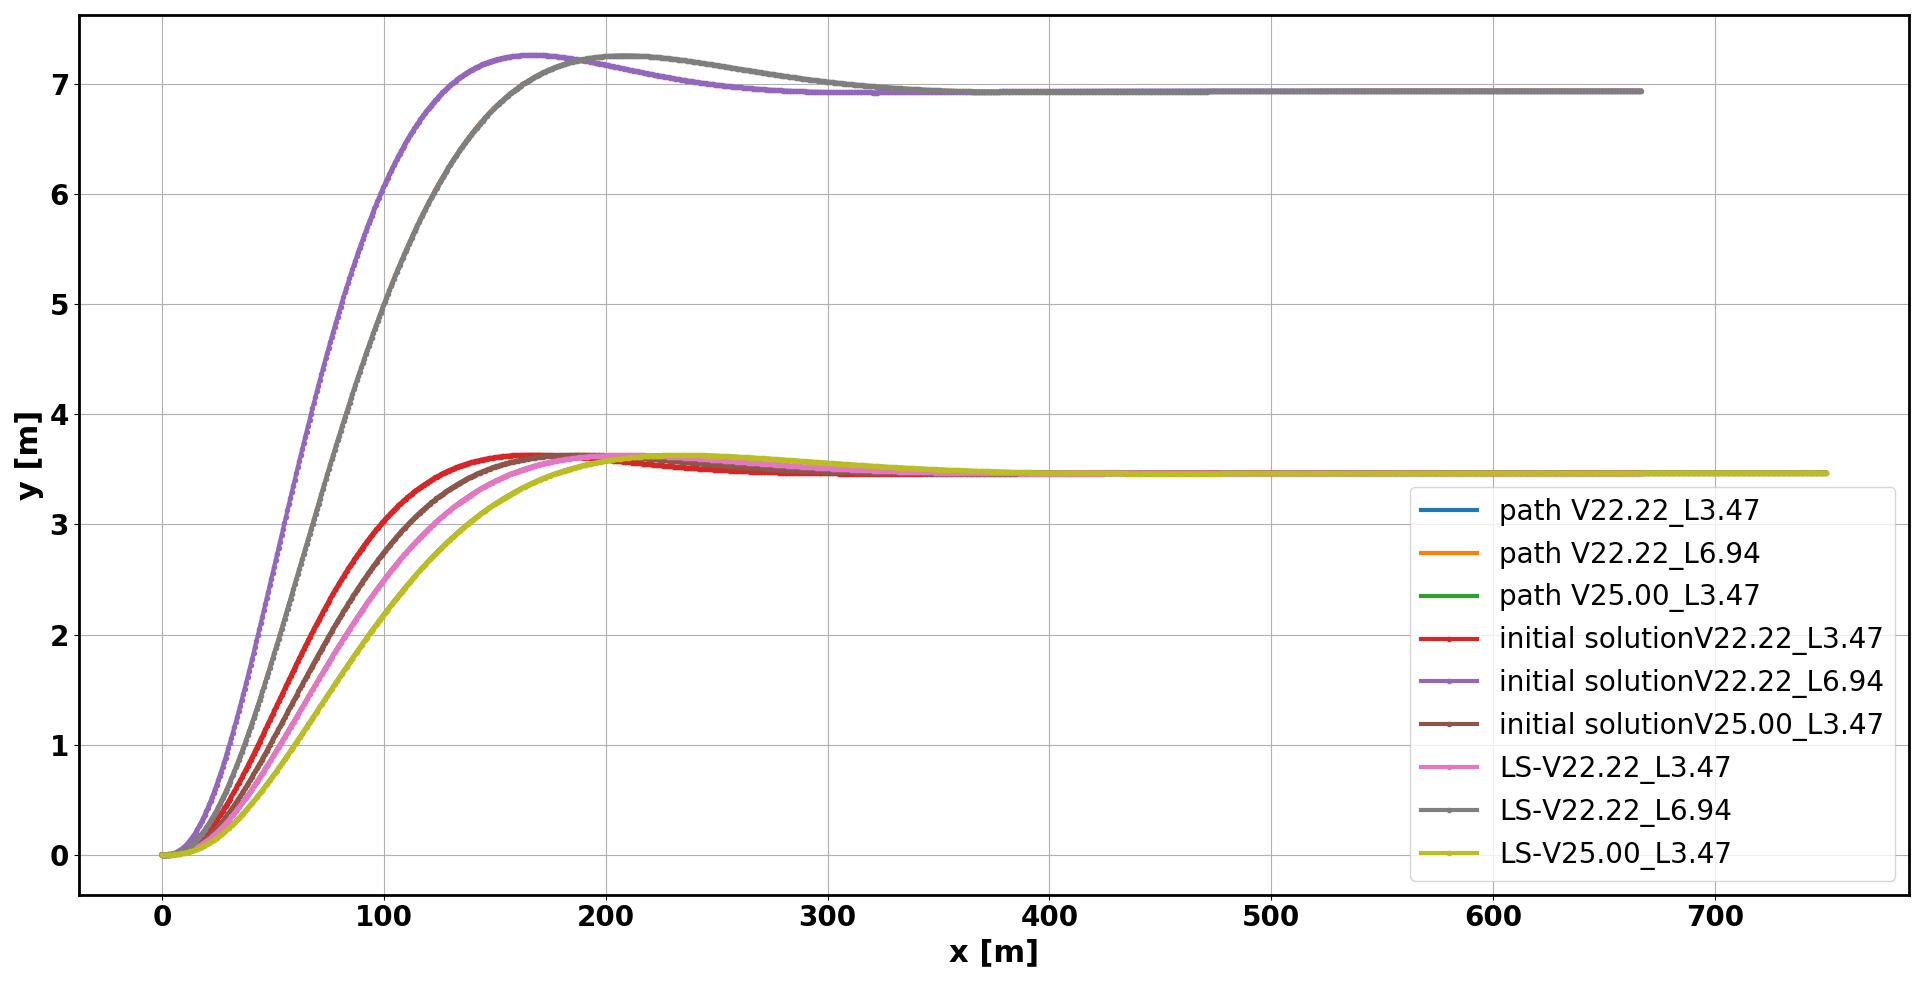
\includegraphics[width=1.0\textwidth]{2l.png}
	\label{fig:lat_acc_val}
\end{figure}

\begin{figure}[h!]
	\centering
	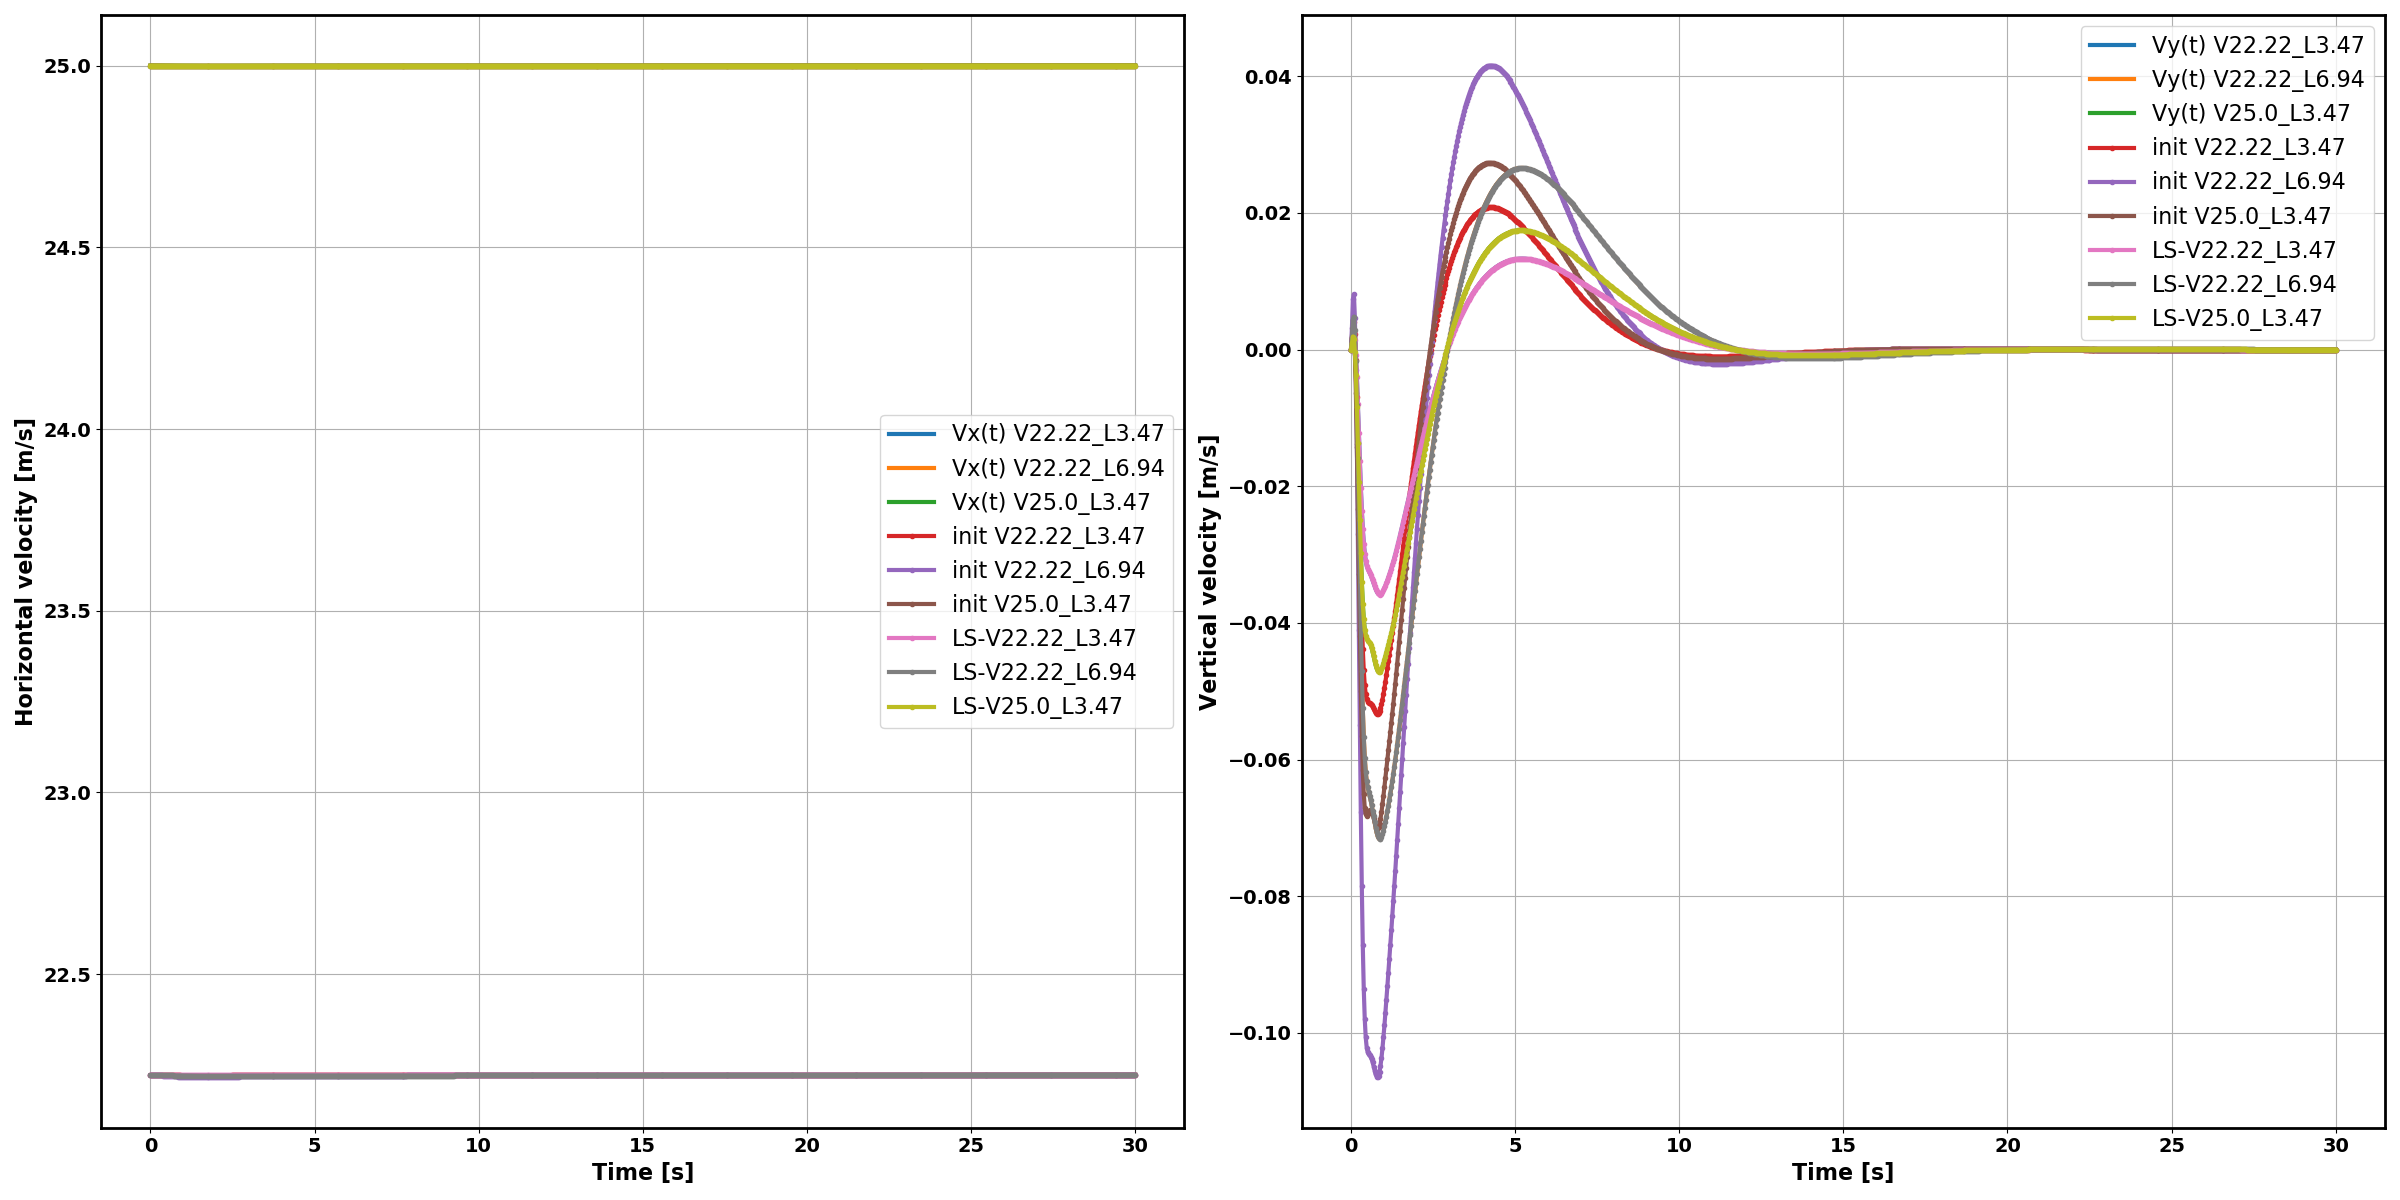
\includegraphics[width=1.0\textwidth]{3l.png}
	\label{fig:lat_acc_val}
\end{figure}


\begin{figure}[h!]
	\centering
	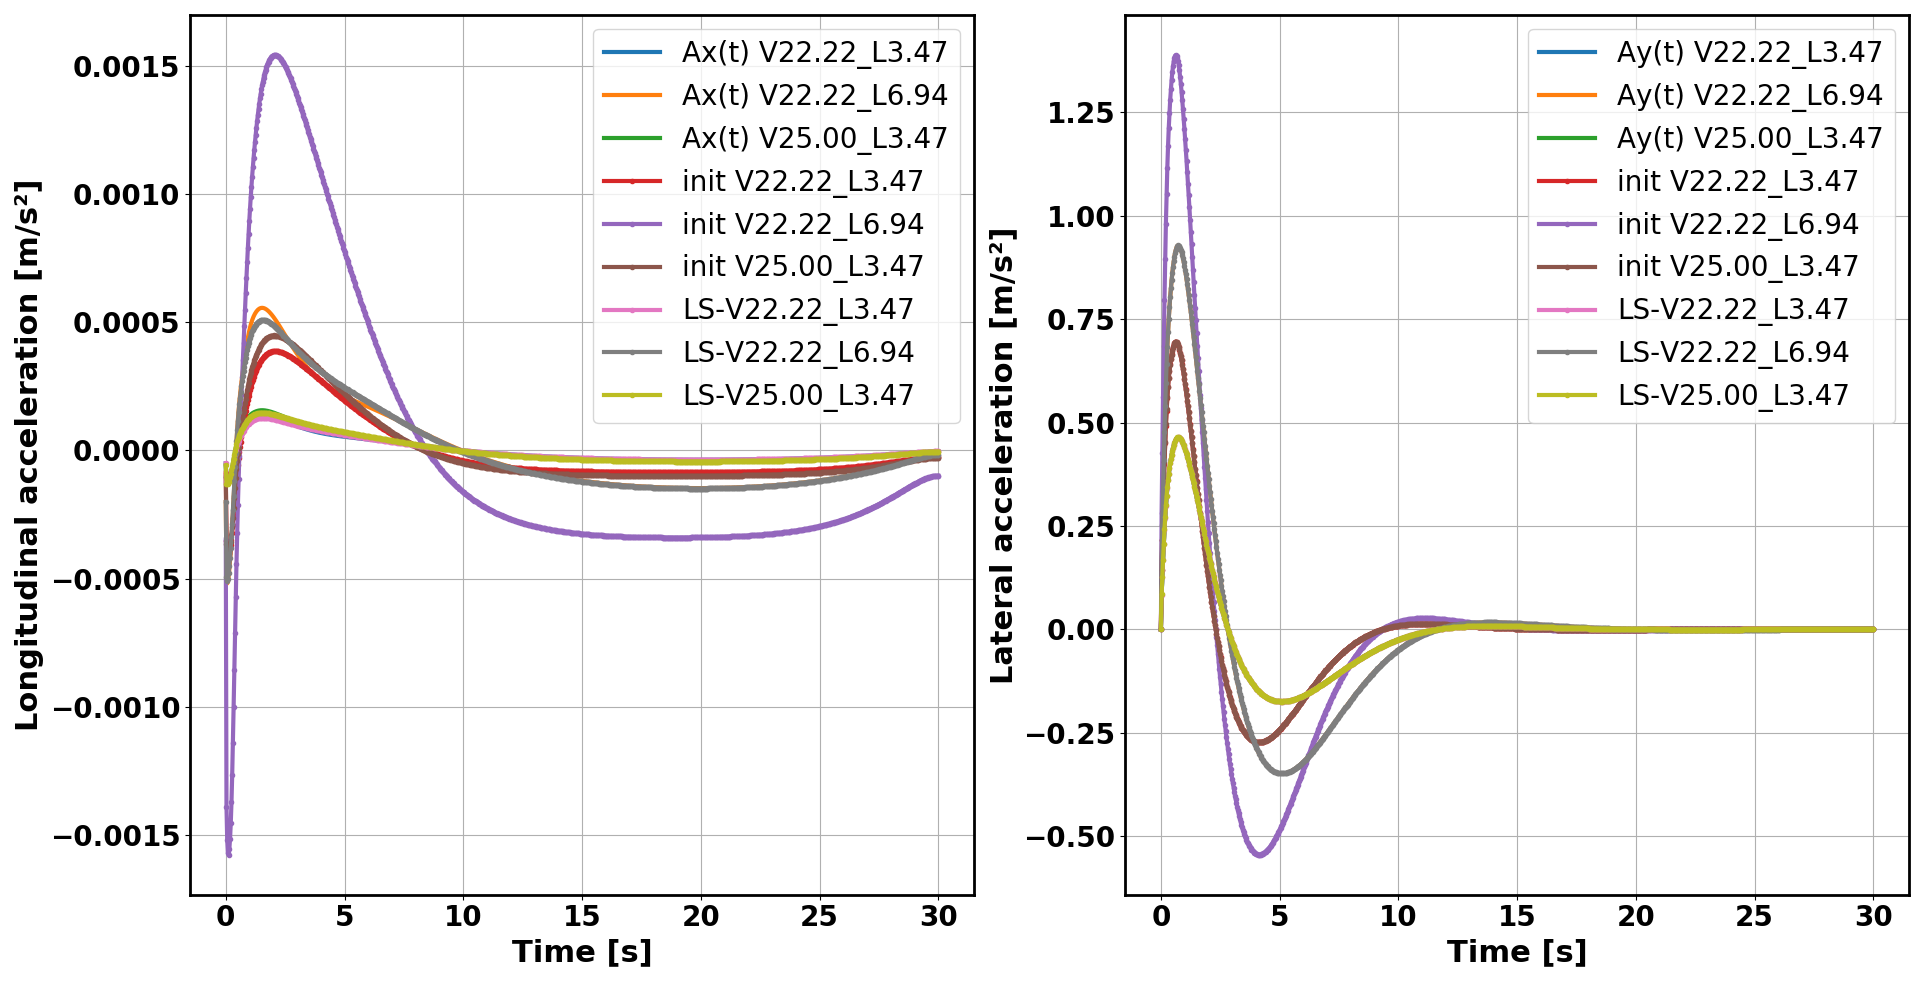
\includegraphics[width=1.0\textwidth]{4l.png}
	\label{fig:lat_acc_val}
\end{figure}


\begin{figure}[h!]
	\centering
	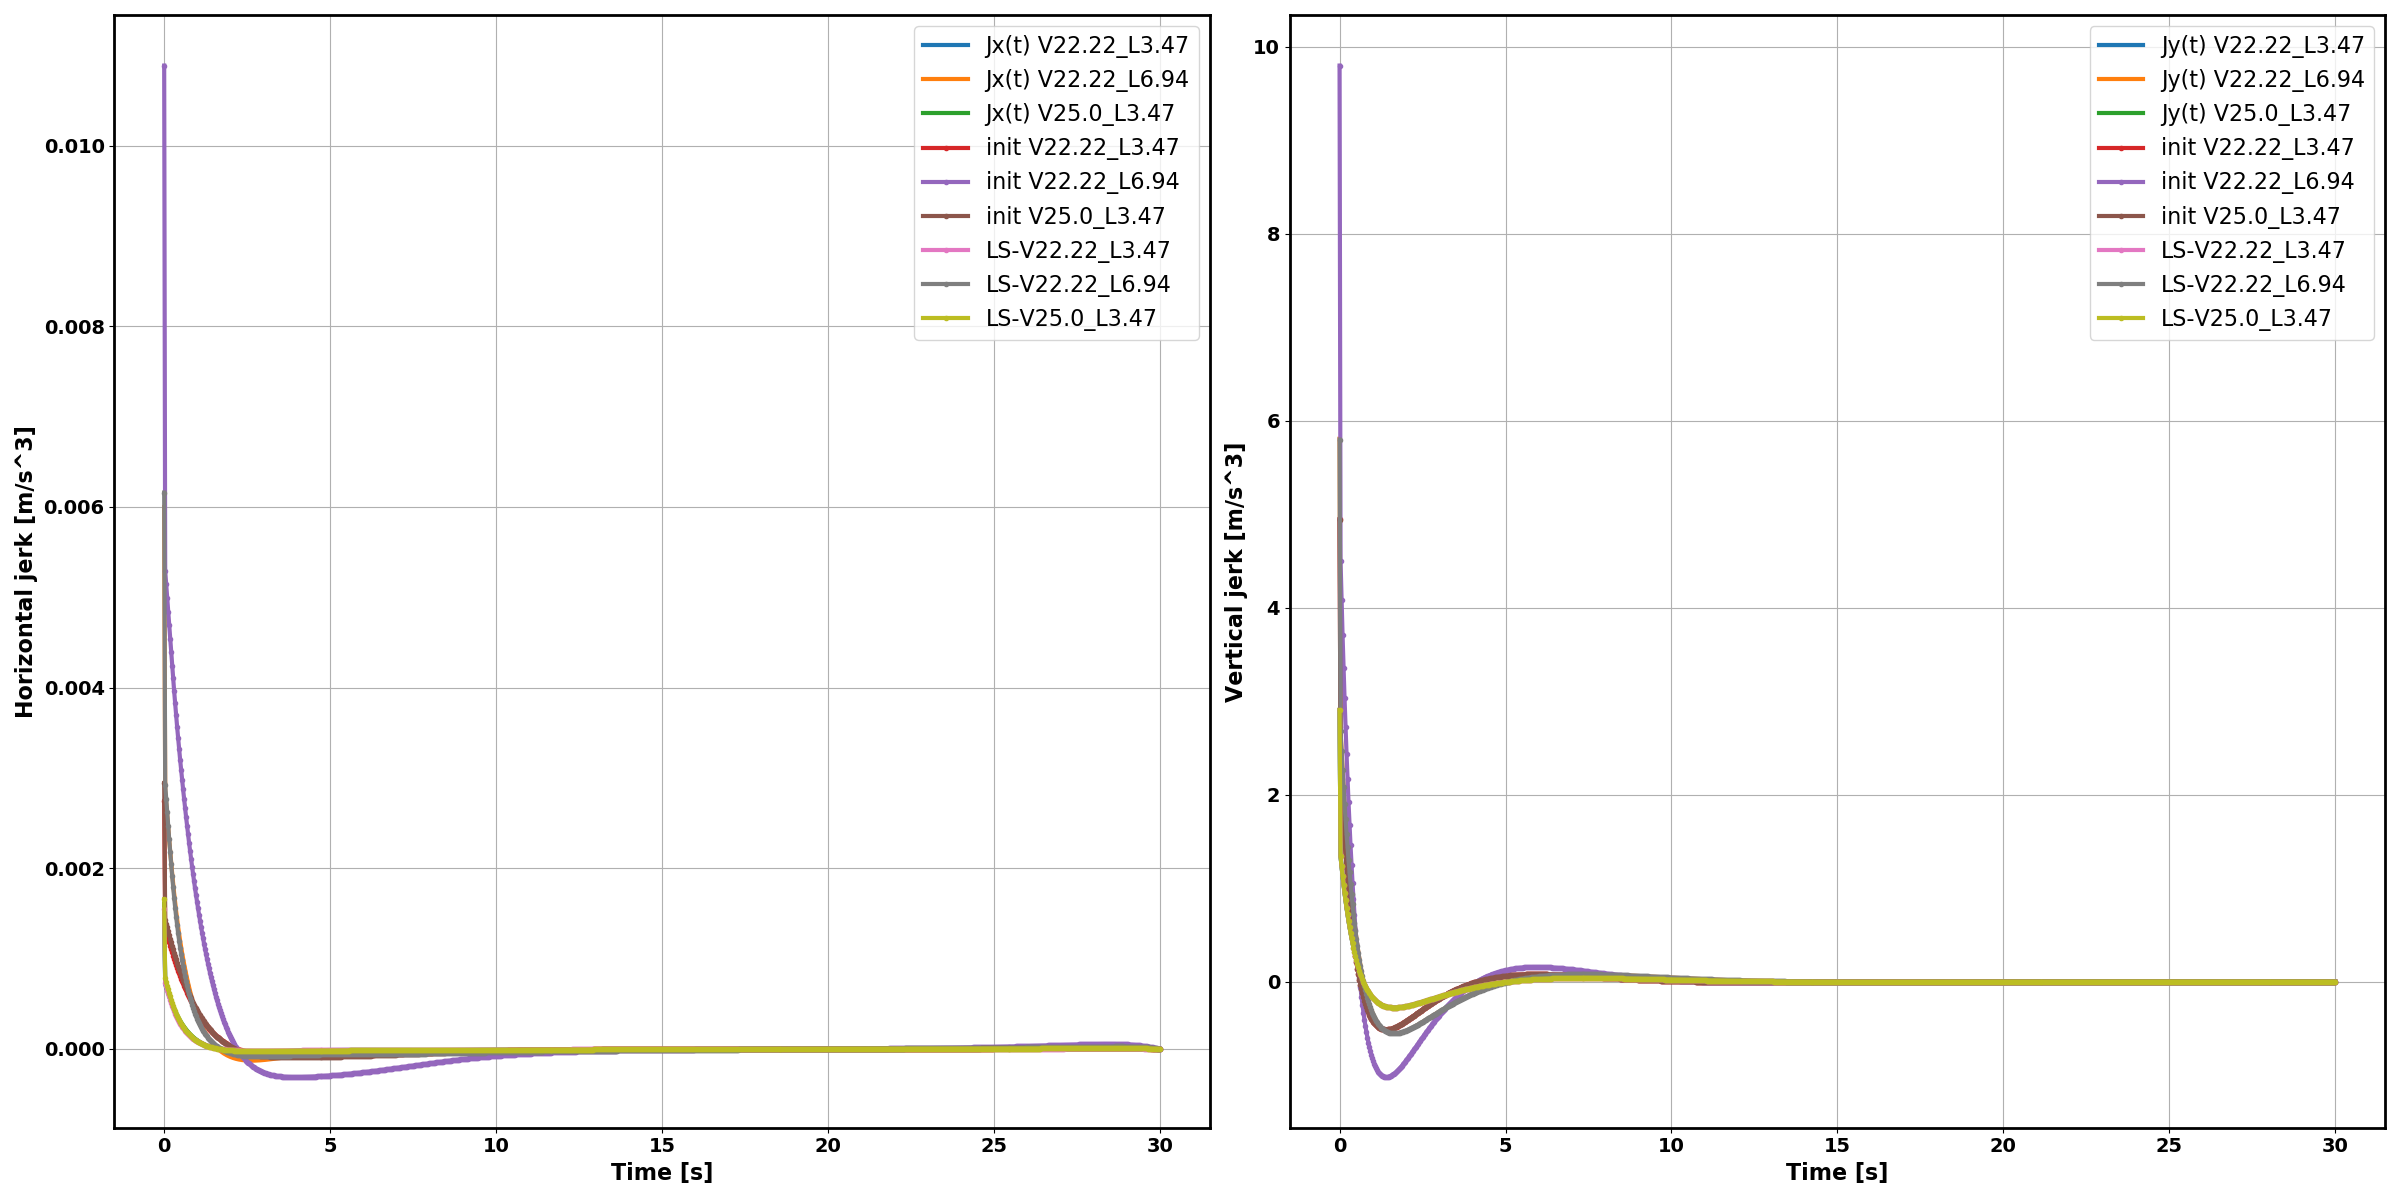
\includegraphics[width=1.0\textwidth]{5l.png}
	\label{fig:lat_acc_val}
\end{figure}


\begin{figure}[h!]
	\centering
	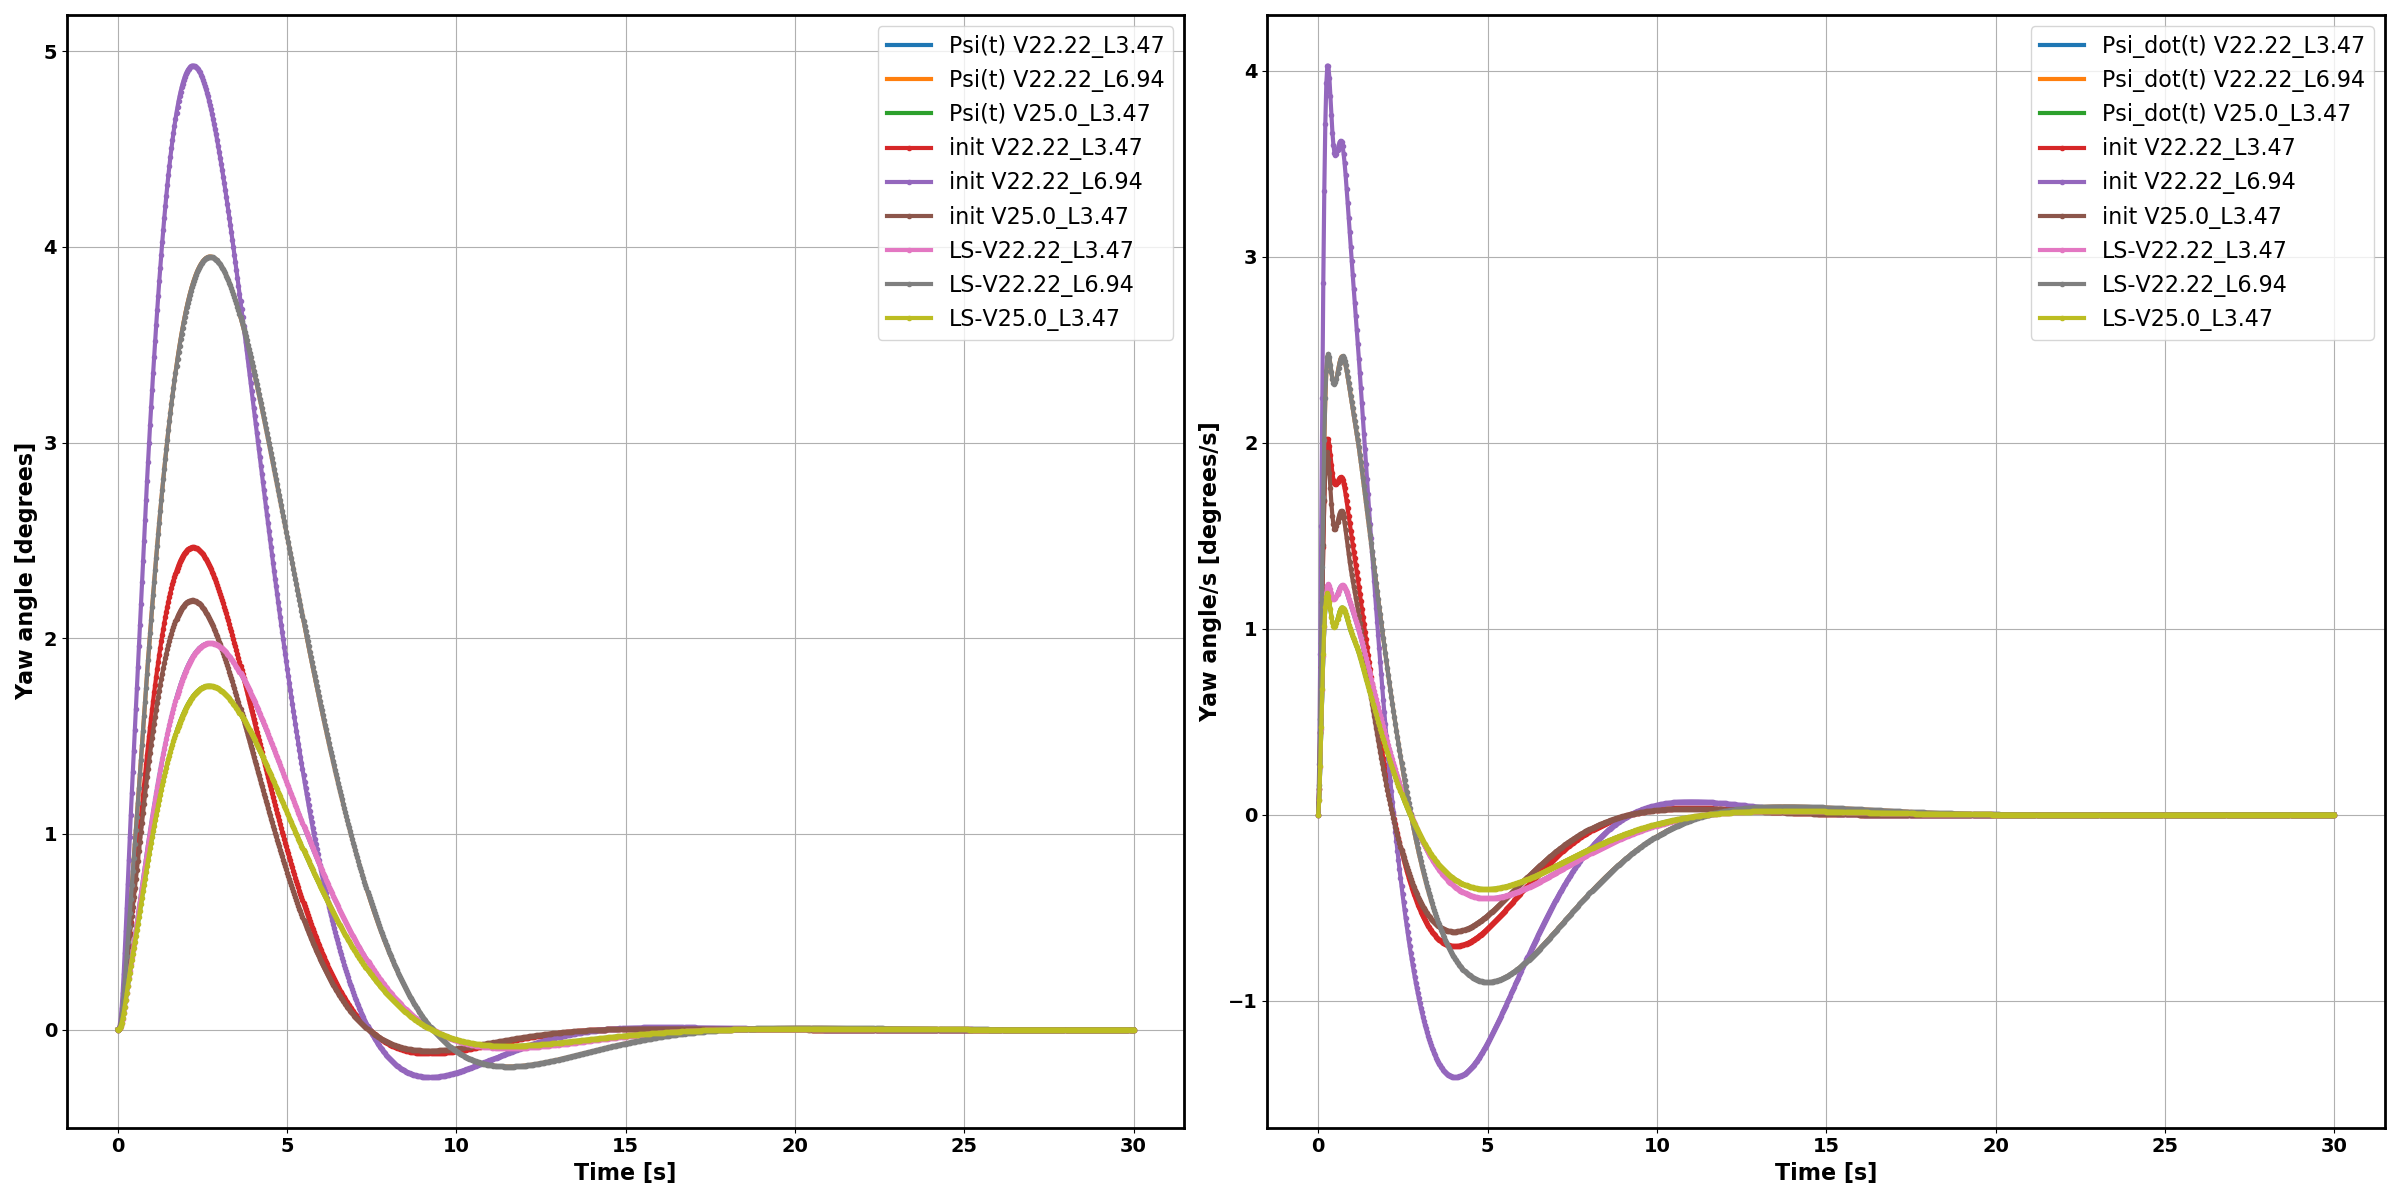
\includegraphics[width=1.0\textwidth]{6l.png}
	\label{fig:lat_acc_val}
\end{figure}


\begin{figure}[h!]
	\centering
	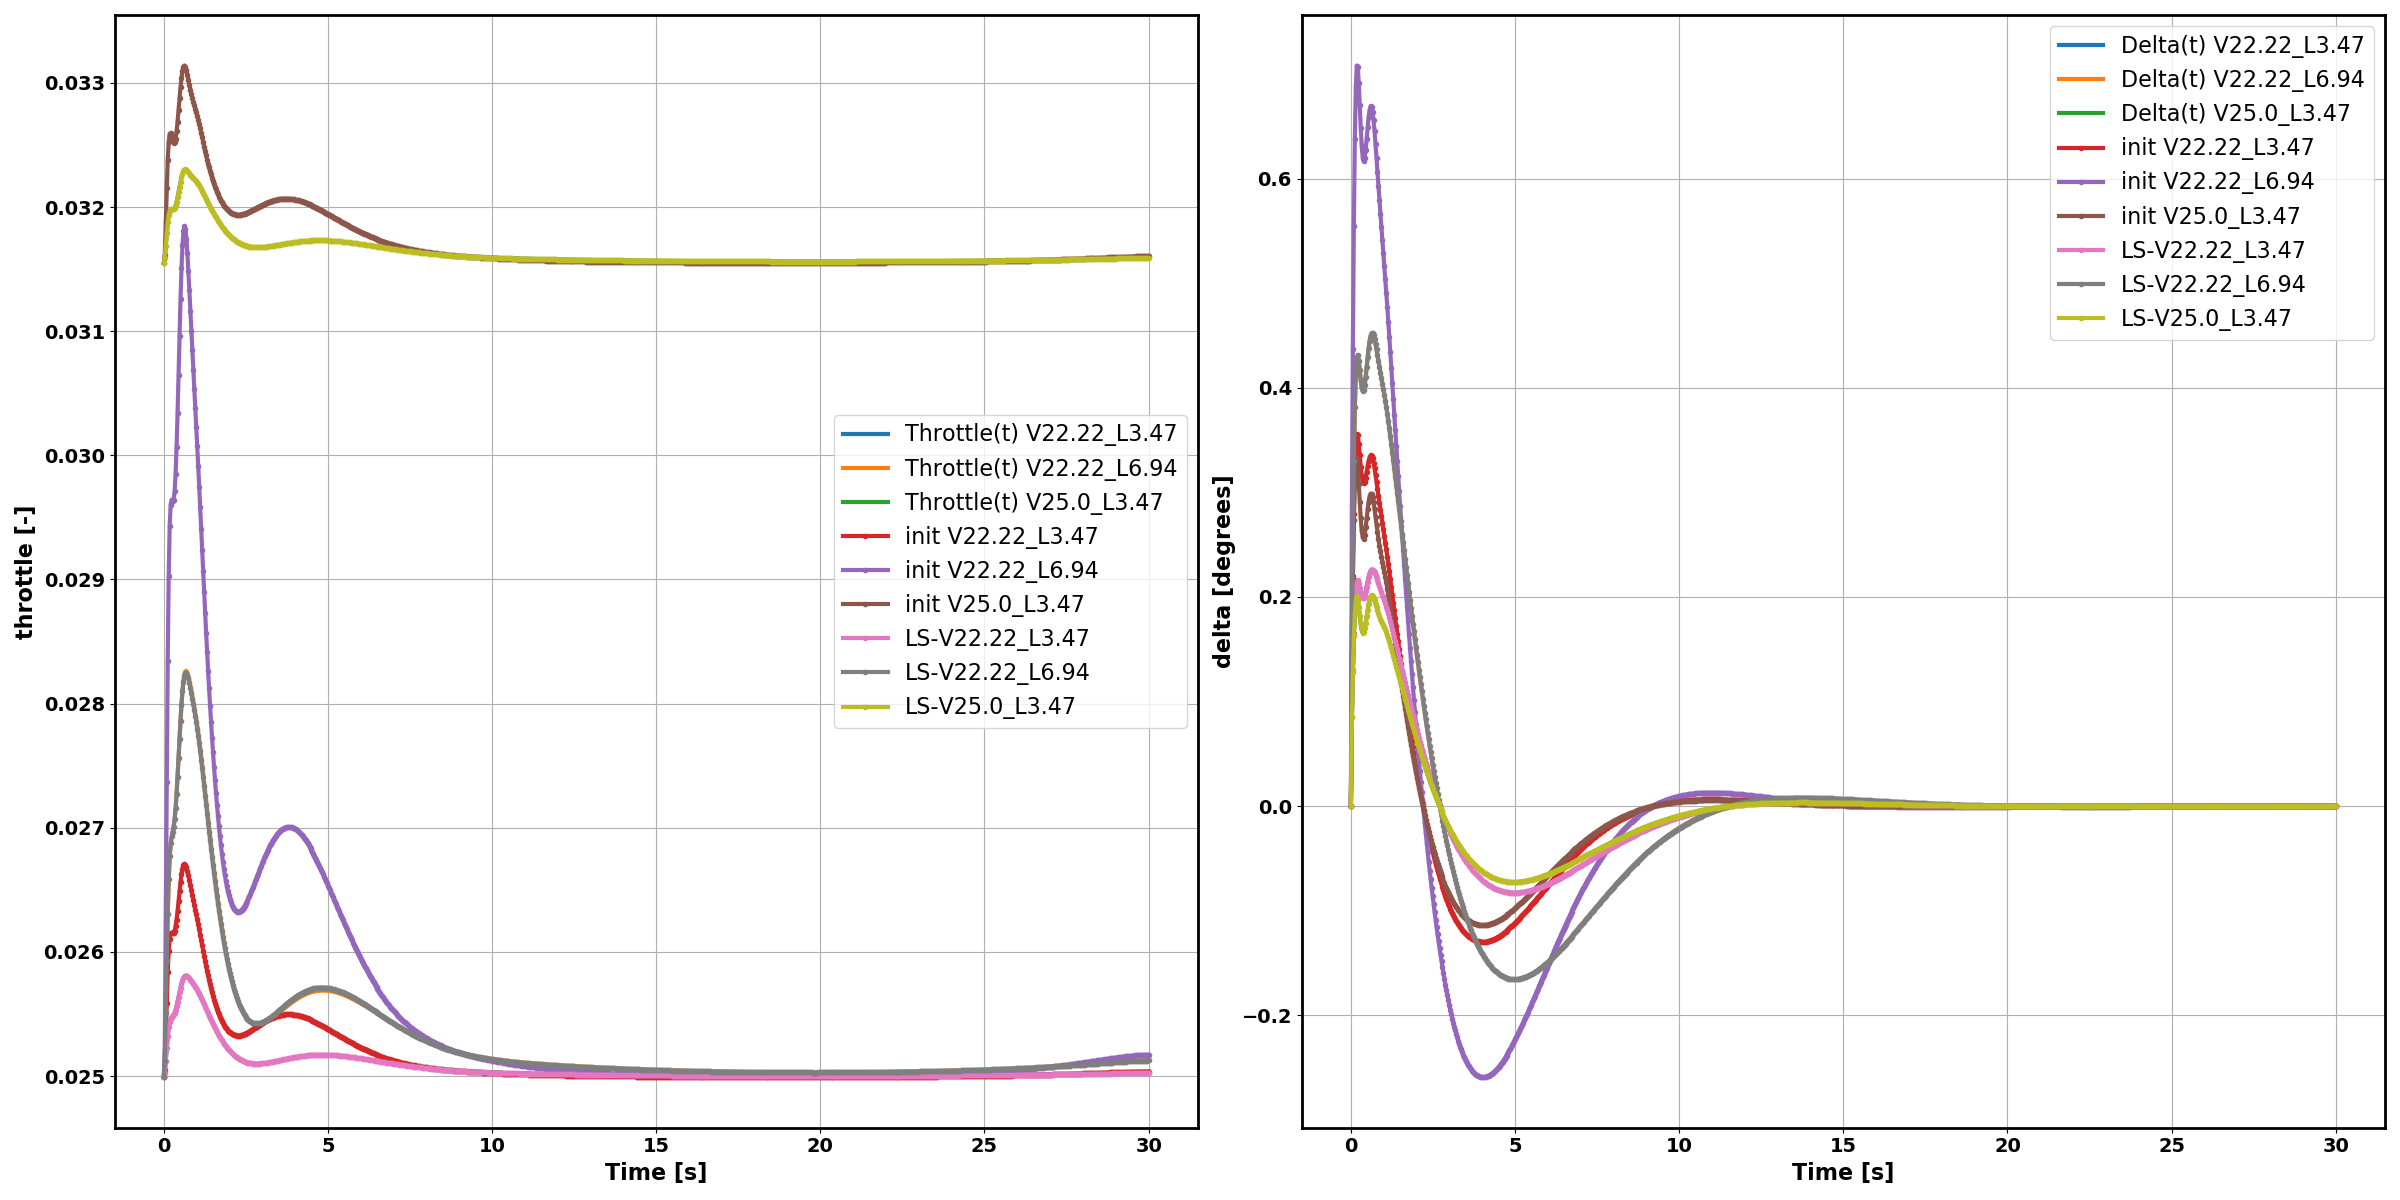
\includegraphics[width=1.0\textwidth]{7l.png}
	\label{fig:lat_acc_val}
\end{figure}


\begin{figure}[h!]
	\centering
	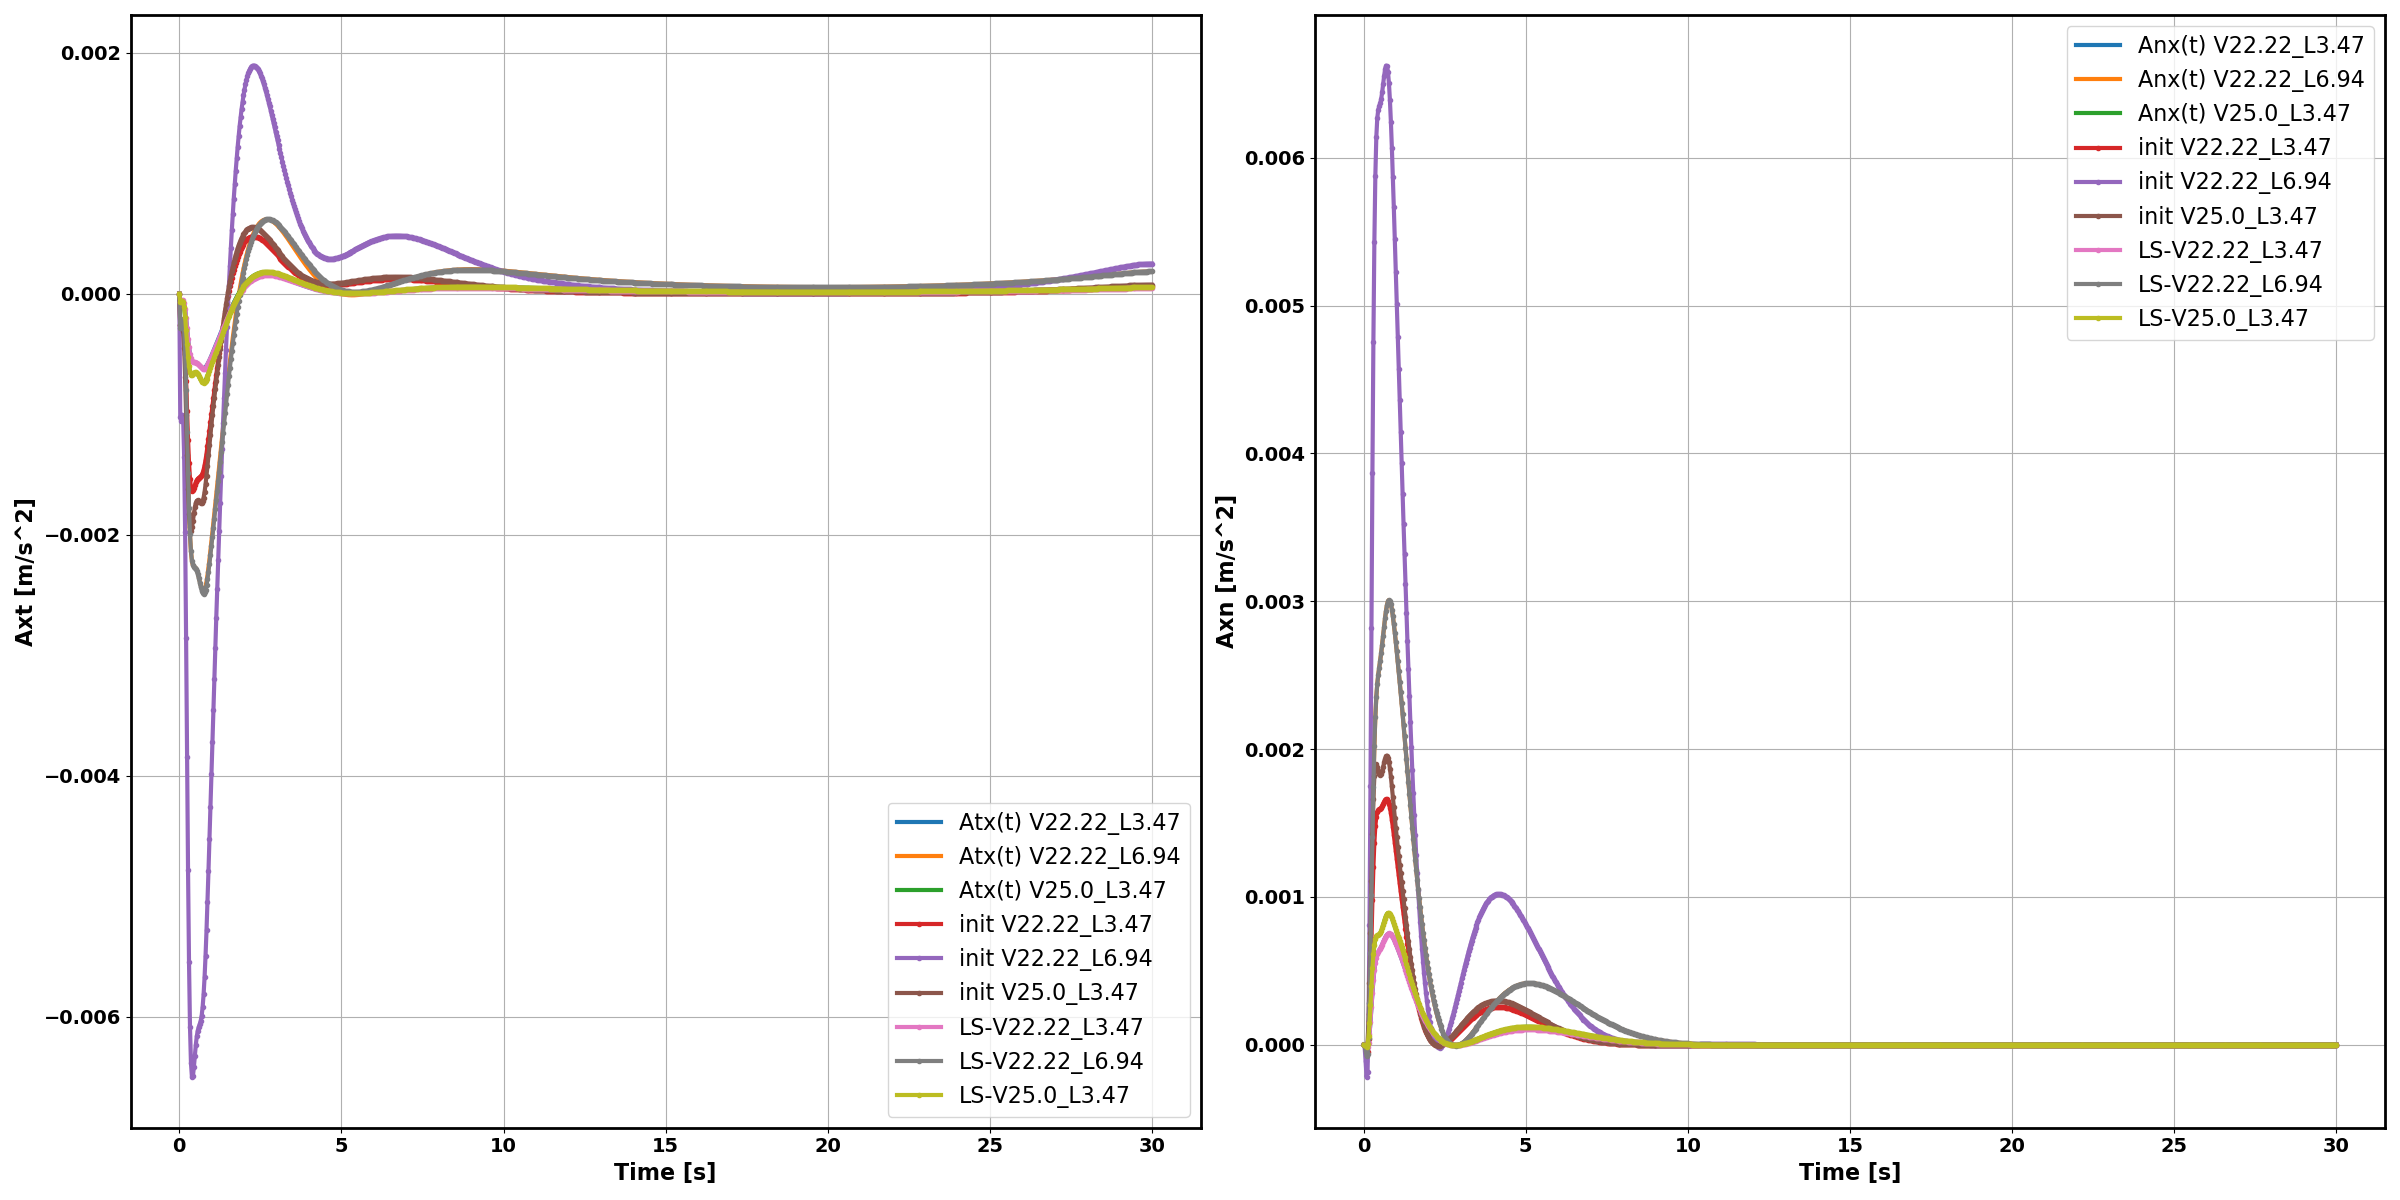
\includegraphics[width=1.0\textwidth]{8l.png}
	\label{fig:lat_acc_val}
\end{figure}


\begin{figure}[h!]
	\centering
	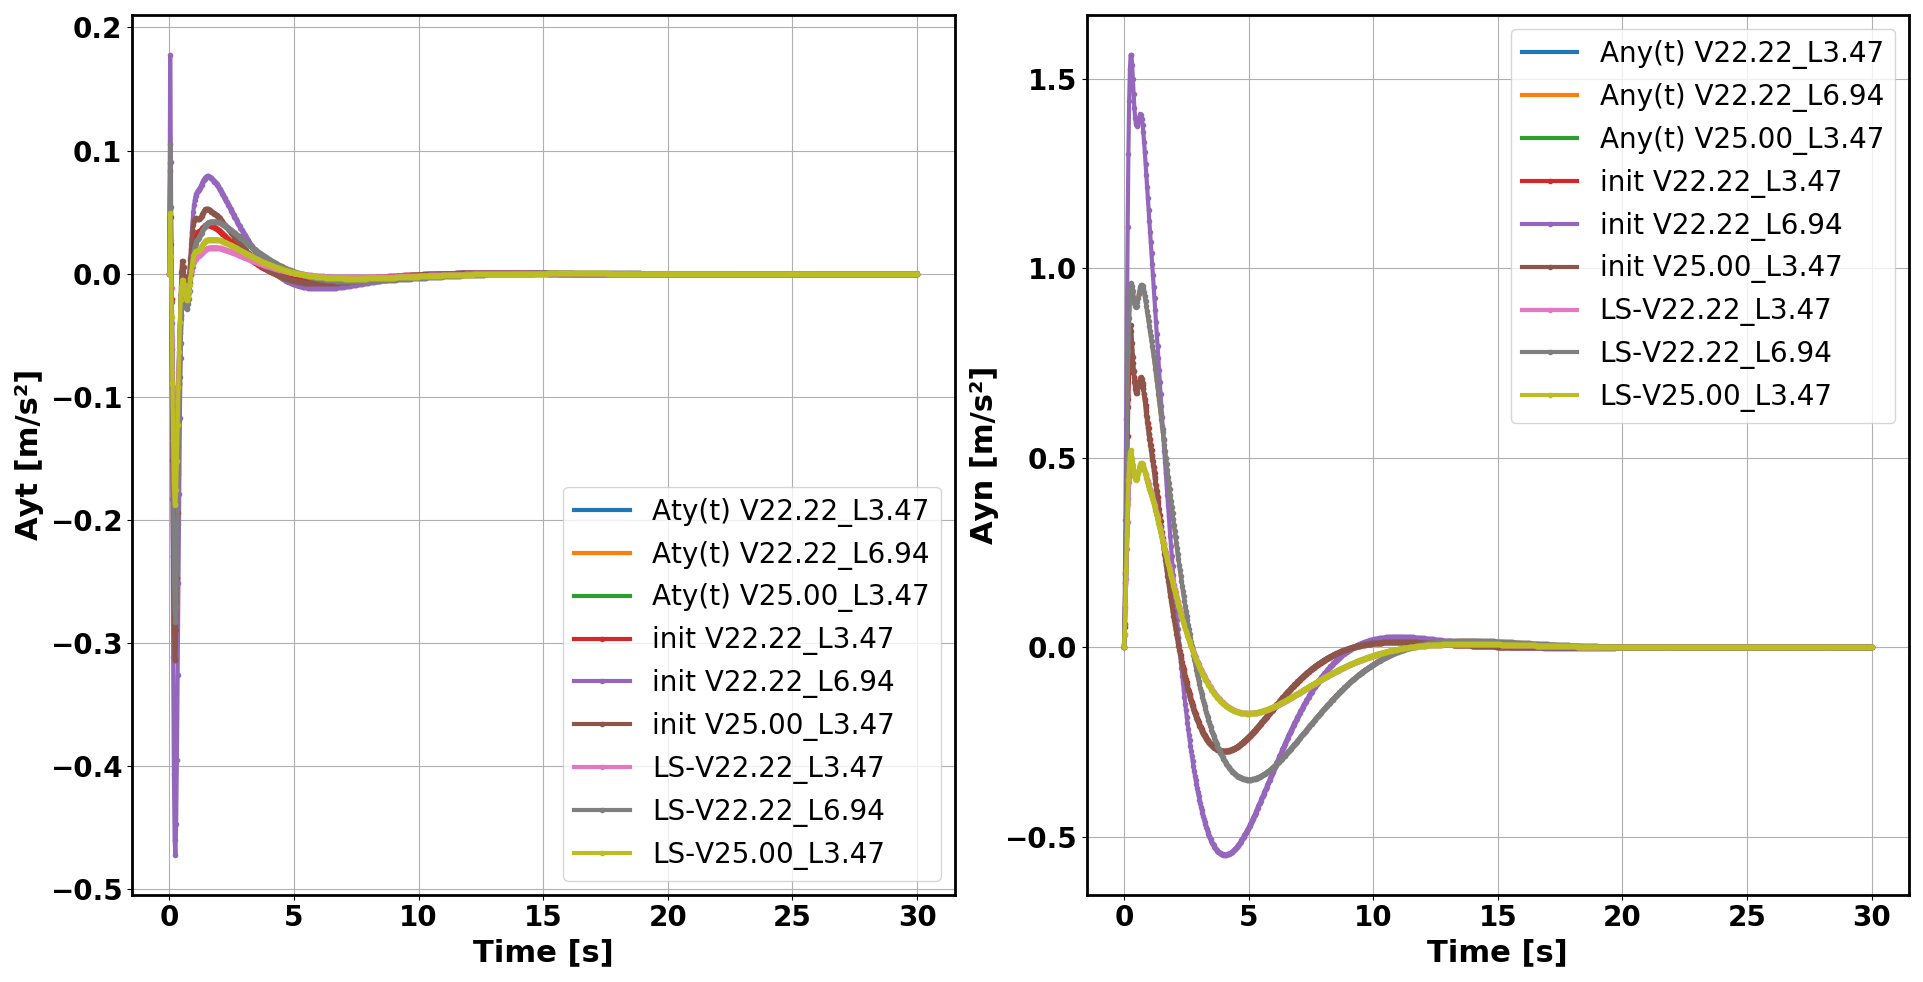
\includegraphics[width=1.0\textwidth]{9l.png}
	\label{fig:lat_acc_val}
\end{figure}


\begin{figure}[h!]
	\centering
	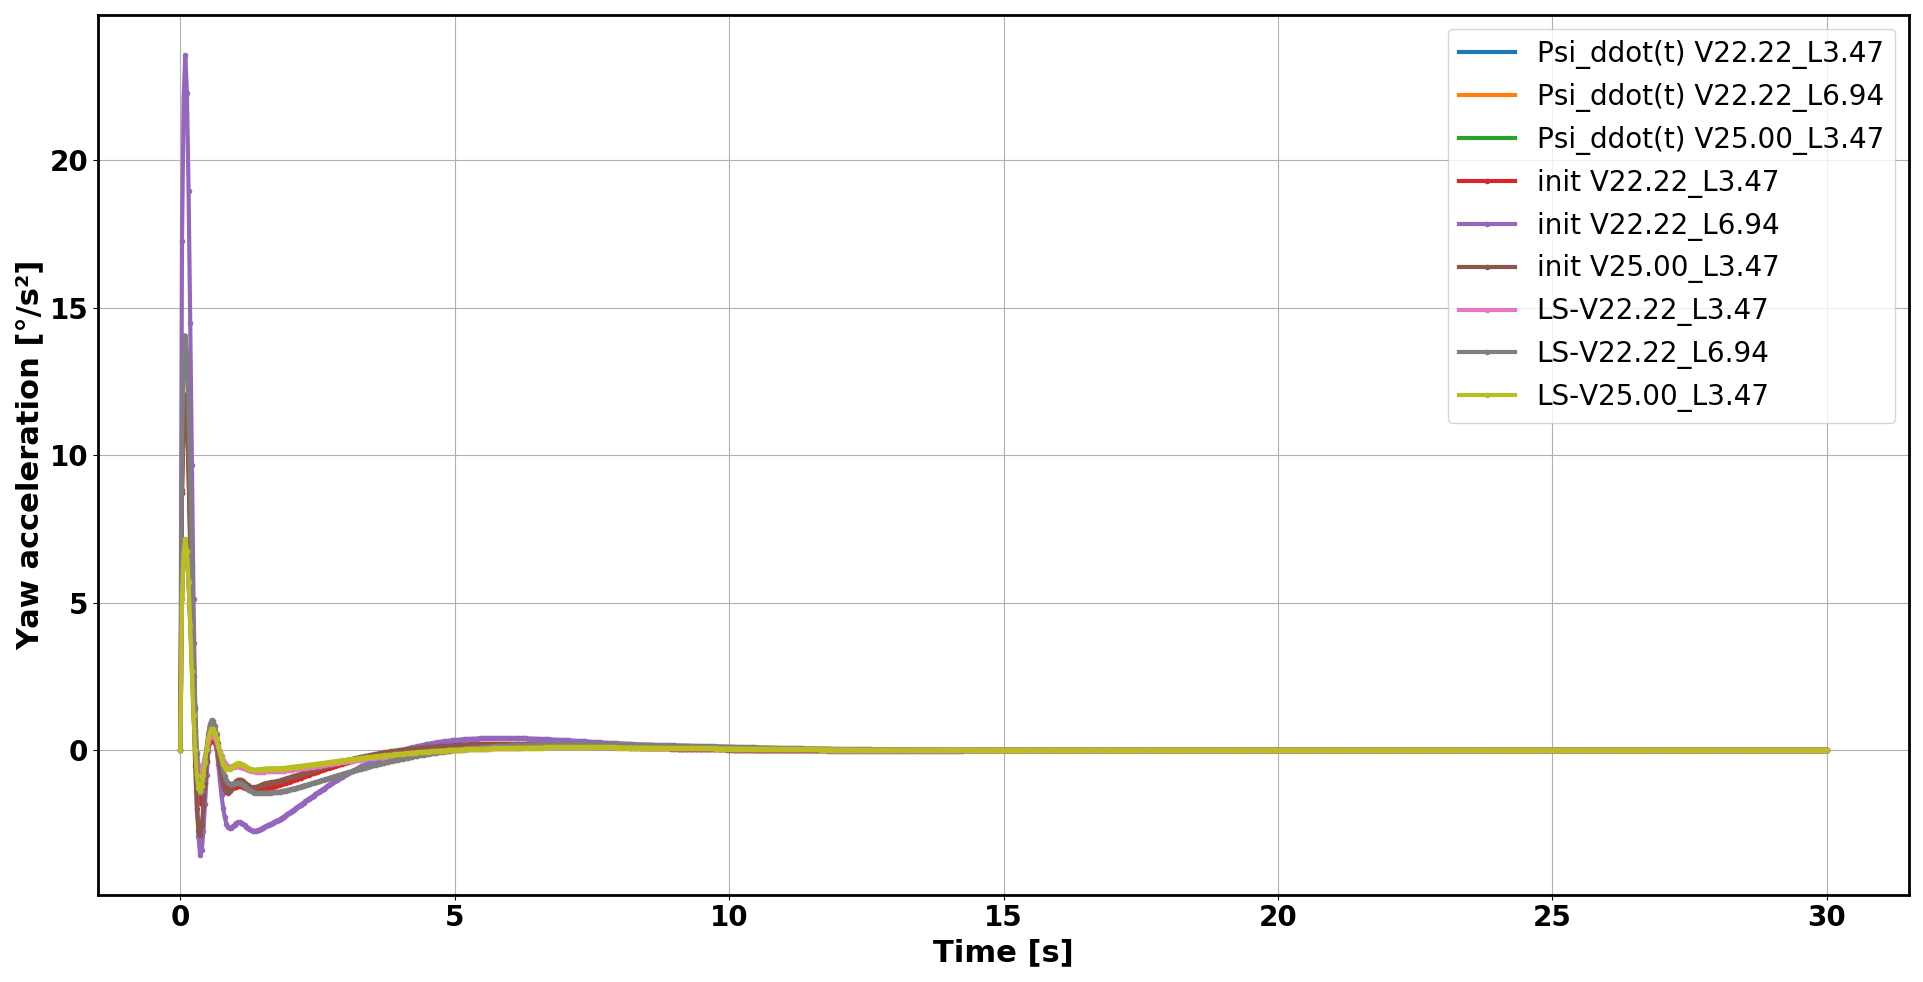
\includegraphics[width=1.0\textwidth]{10l.png}
	\label{fig:lat_acc_val}
\end{figure}


\begin{figure}[h!]
	\centering
	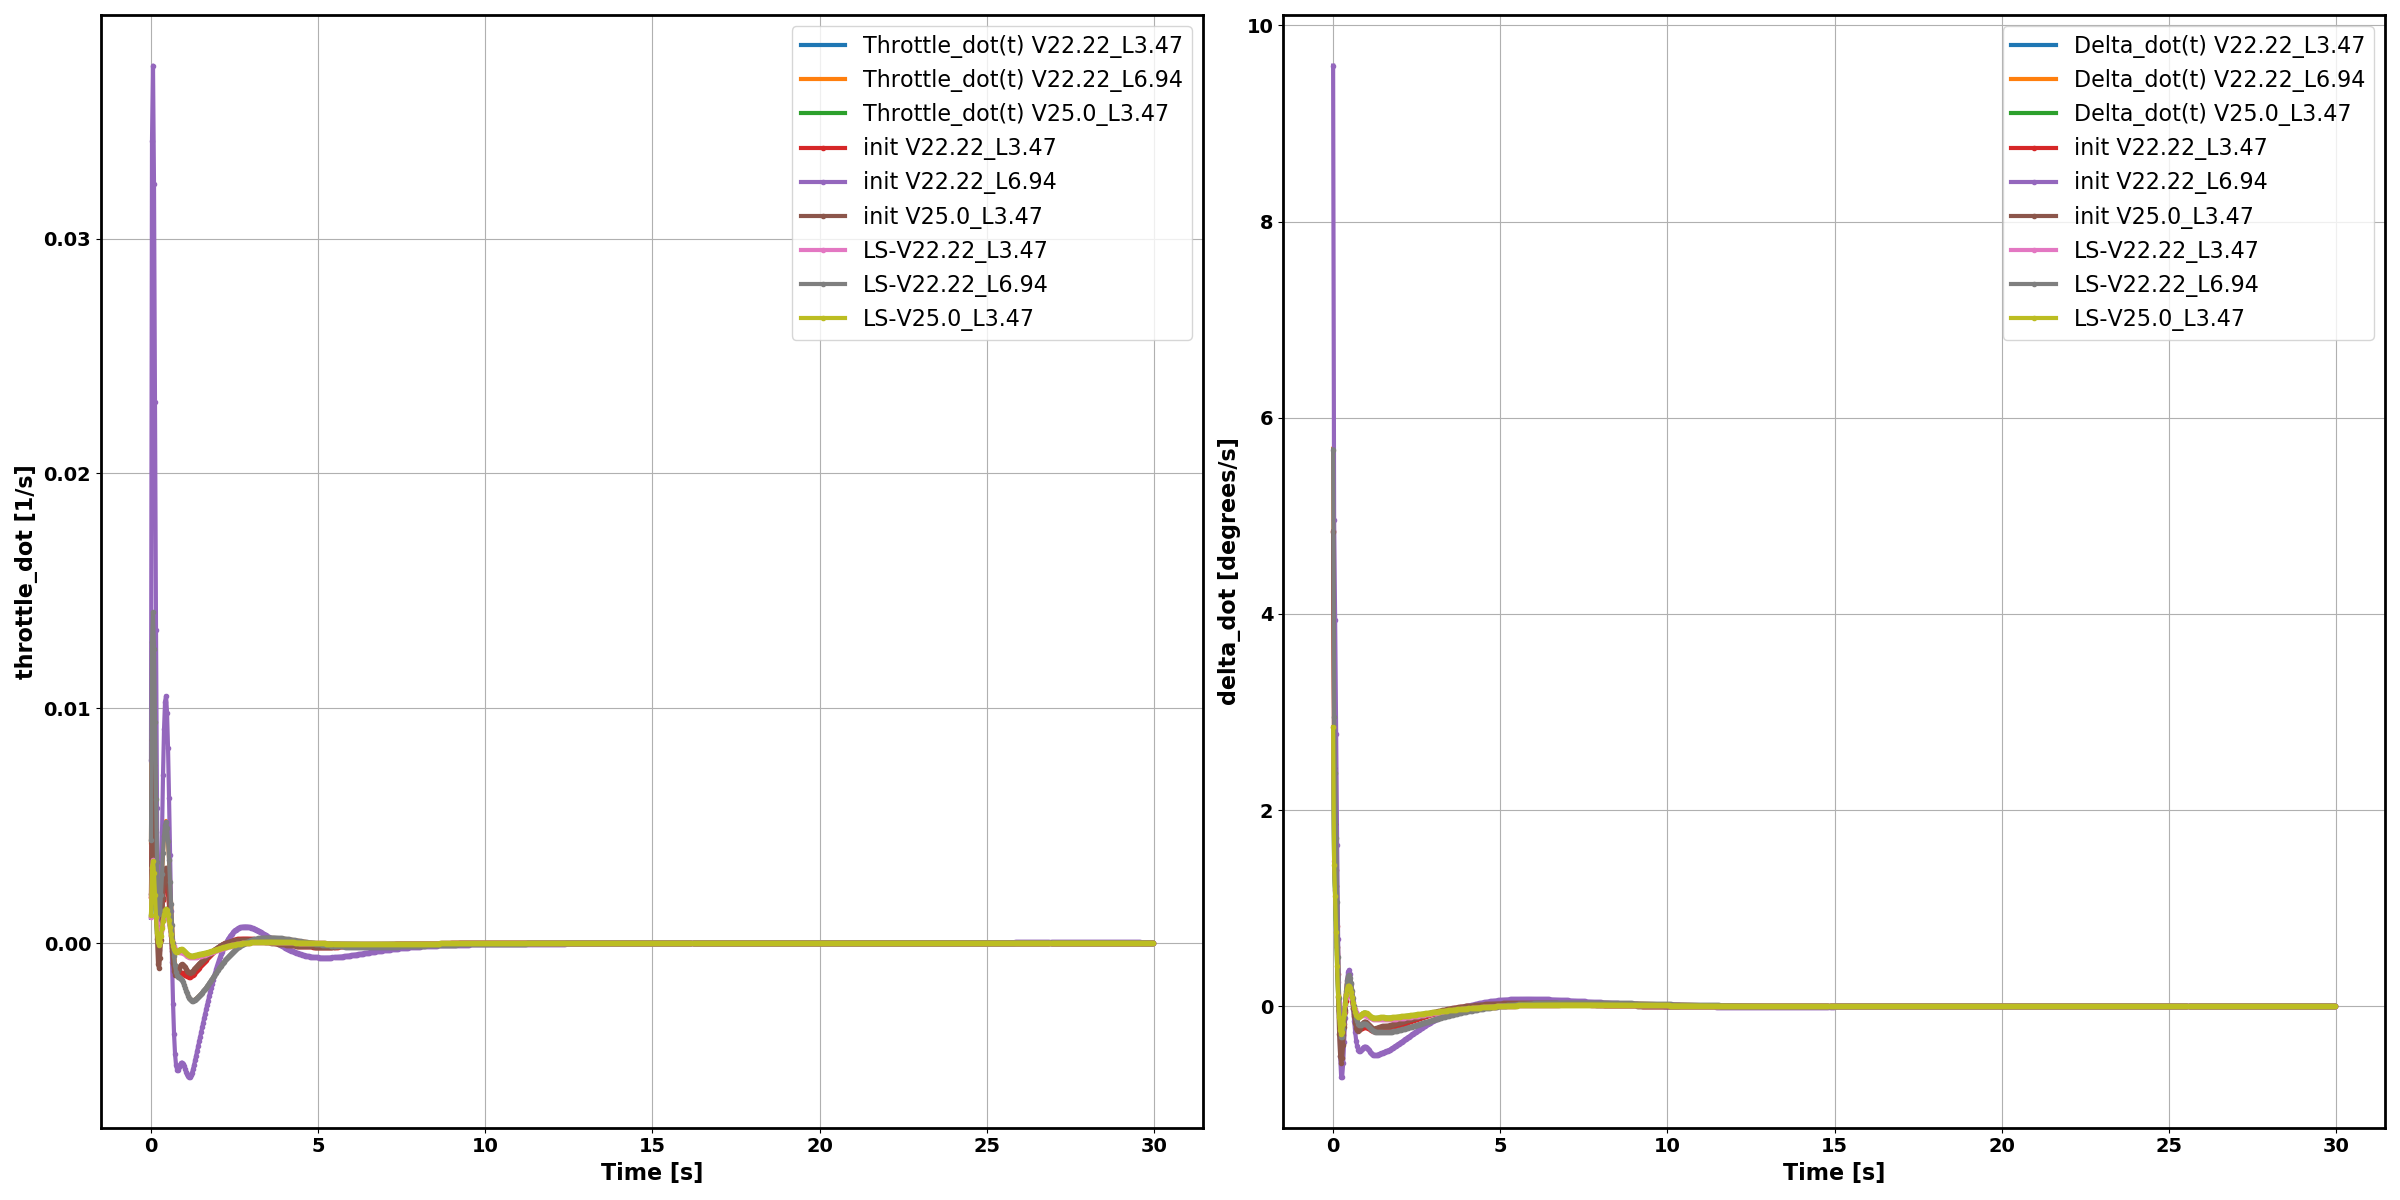
\includegraphics[width=1.0\textwidth]{11l.png}
	\label{fig:lat_acc_val}
\end{figure}



\begin{figure}[h!]\label{fig:app_conv}
	\centering
	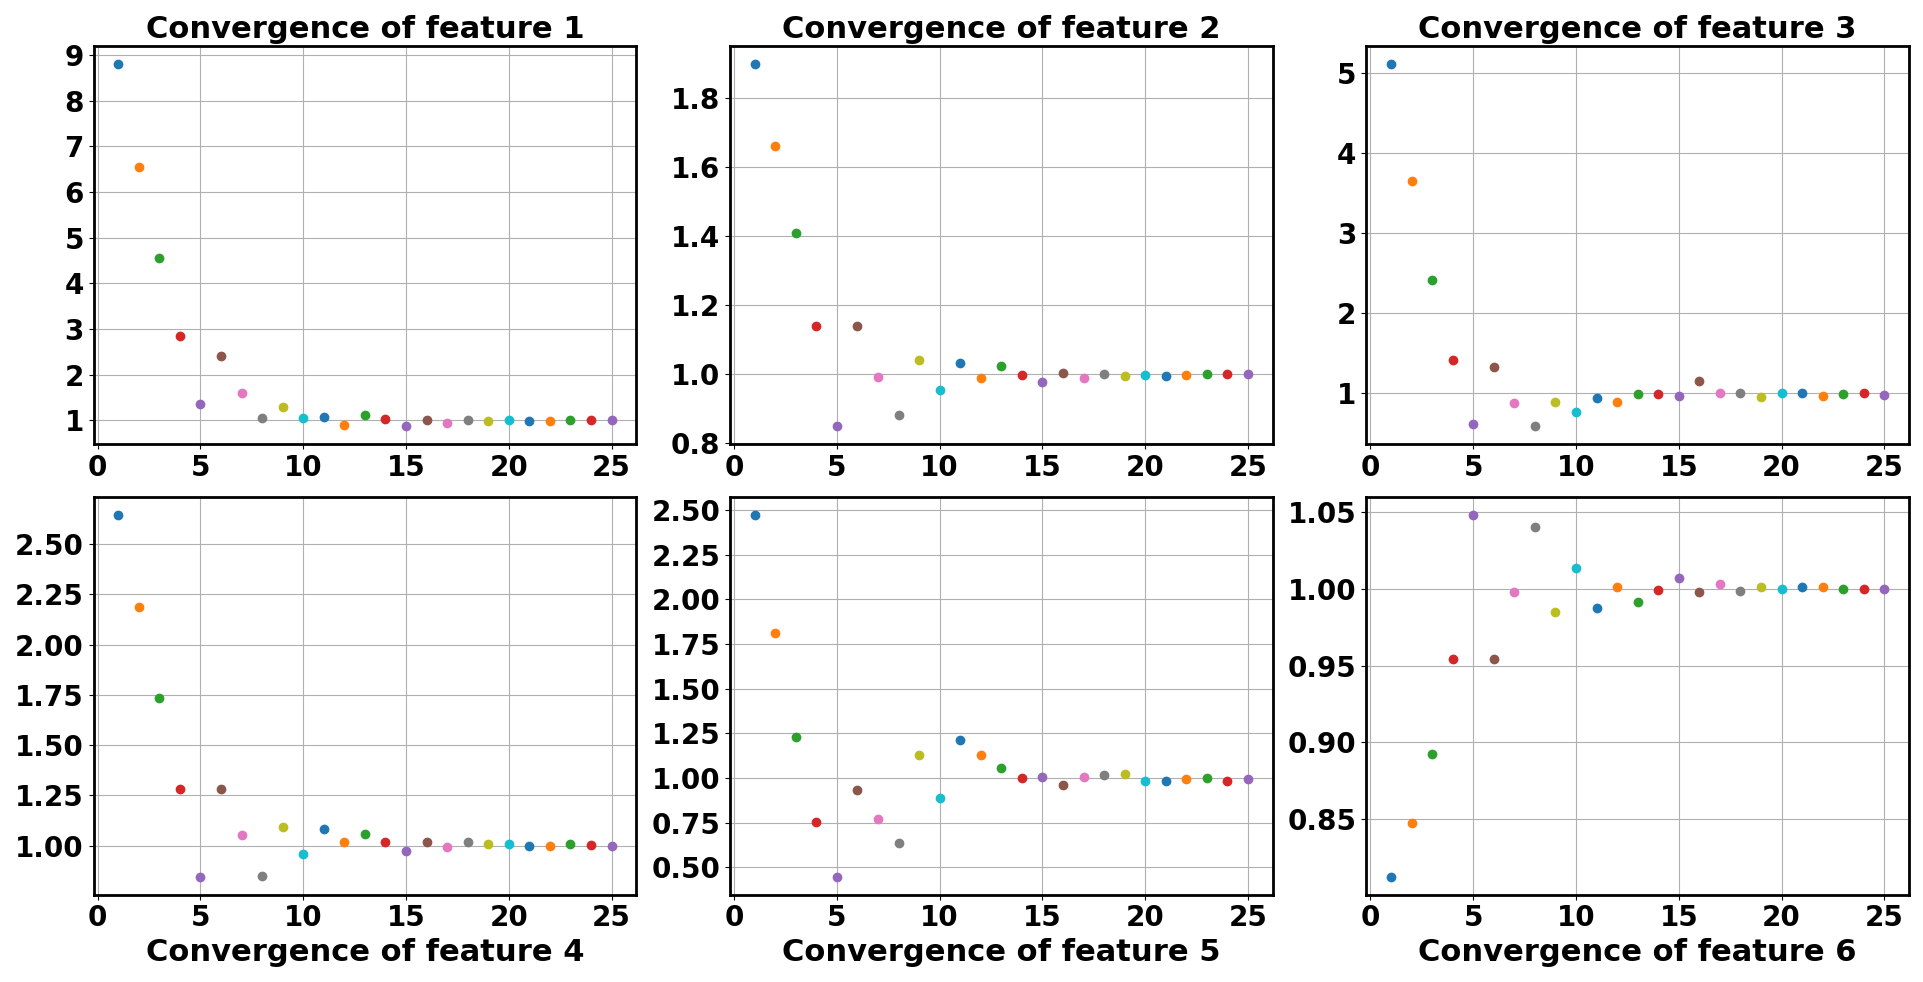
\includegraphics[width=1.0\textwidth]{12l.png}	
	\caption{}
\end{figure}


\begin{figure}[h!]\label{fig:app_grad}
	\centering
	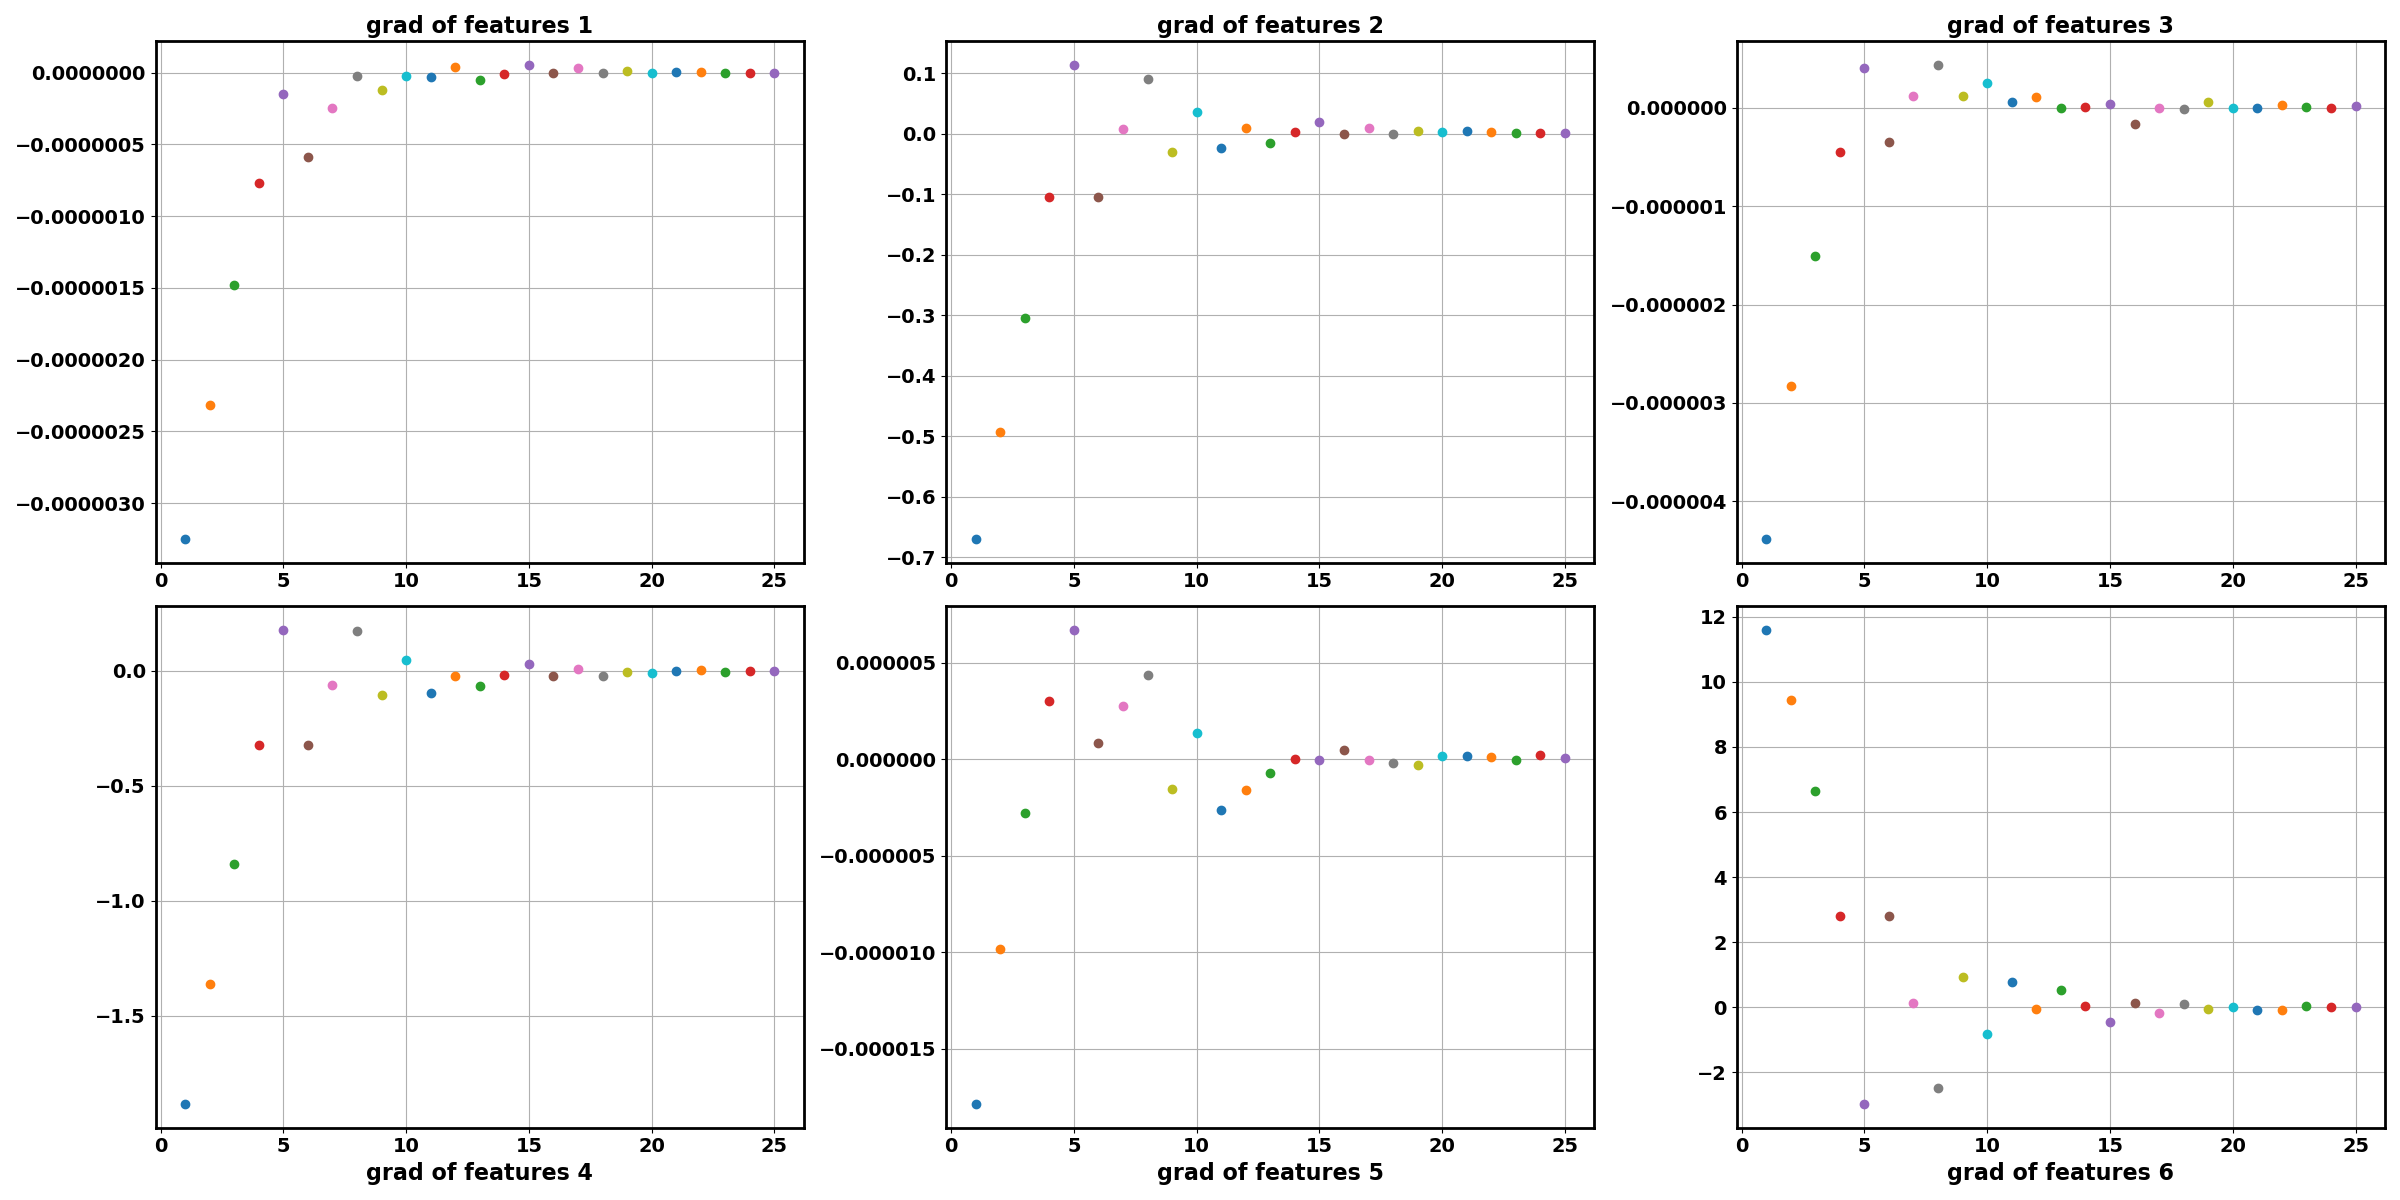
\includegraphics[width=1.0\textwidth]{13l.png}
	\caption{}
	
\end{figure}

\begin{figure}[h!]\label{fig:app_weights}
	\centering
	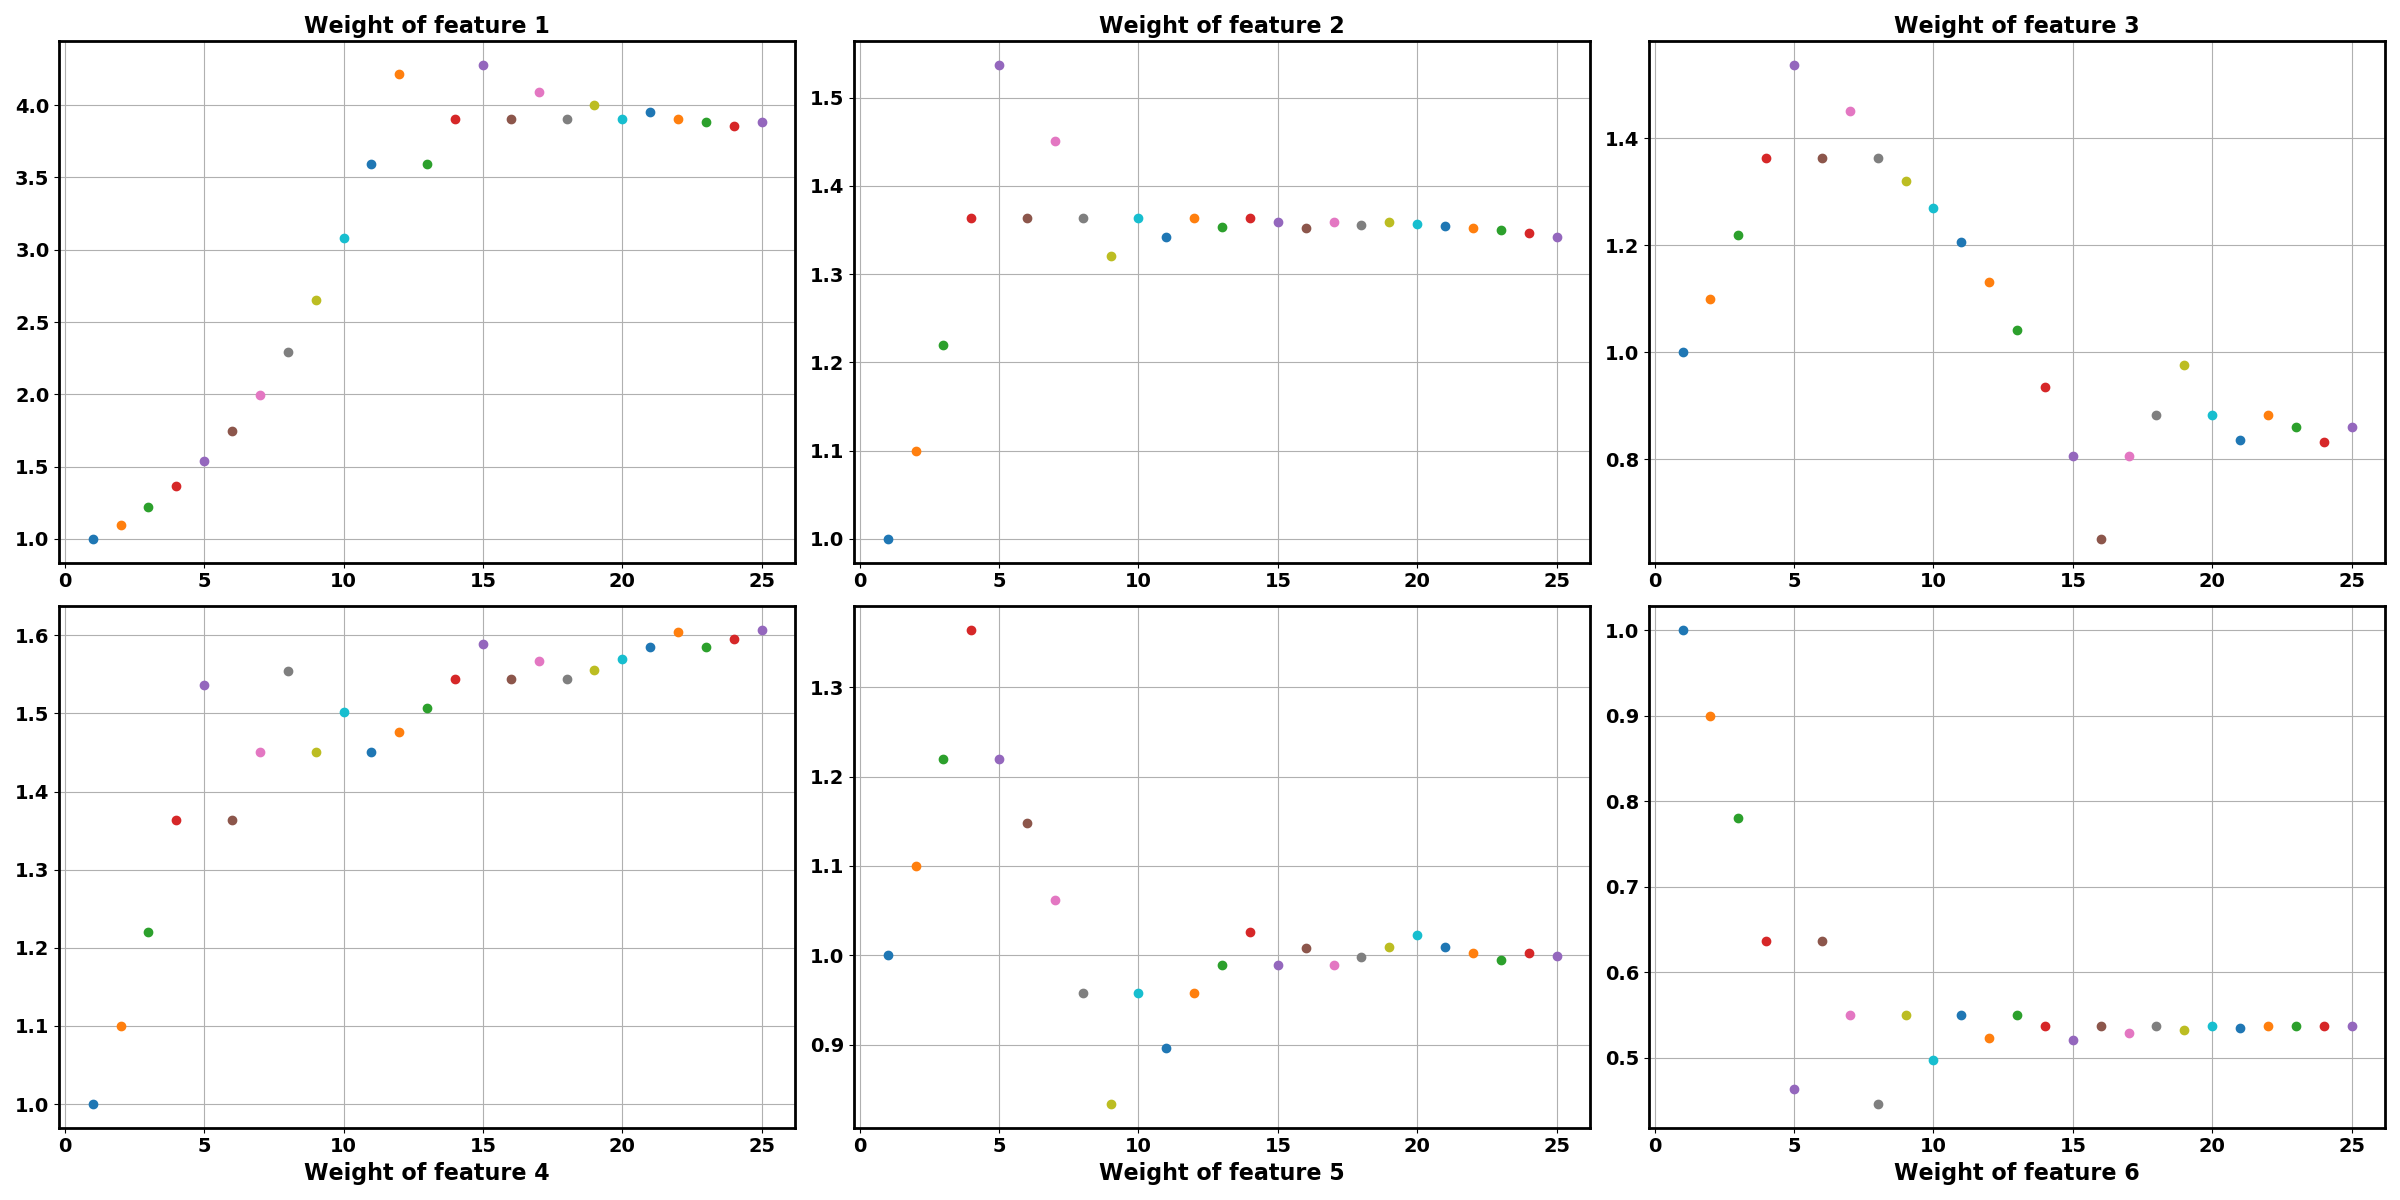
\includegraphics[width=1.0\textwidth]{14l.png}
	\caption{}
	
\end{figure}


\begin{figure}[h!]\label{fig:app_update}
	\centering
	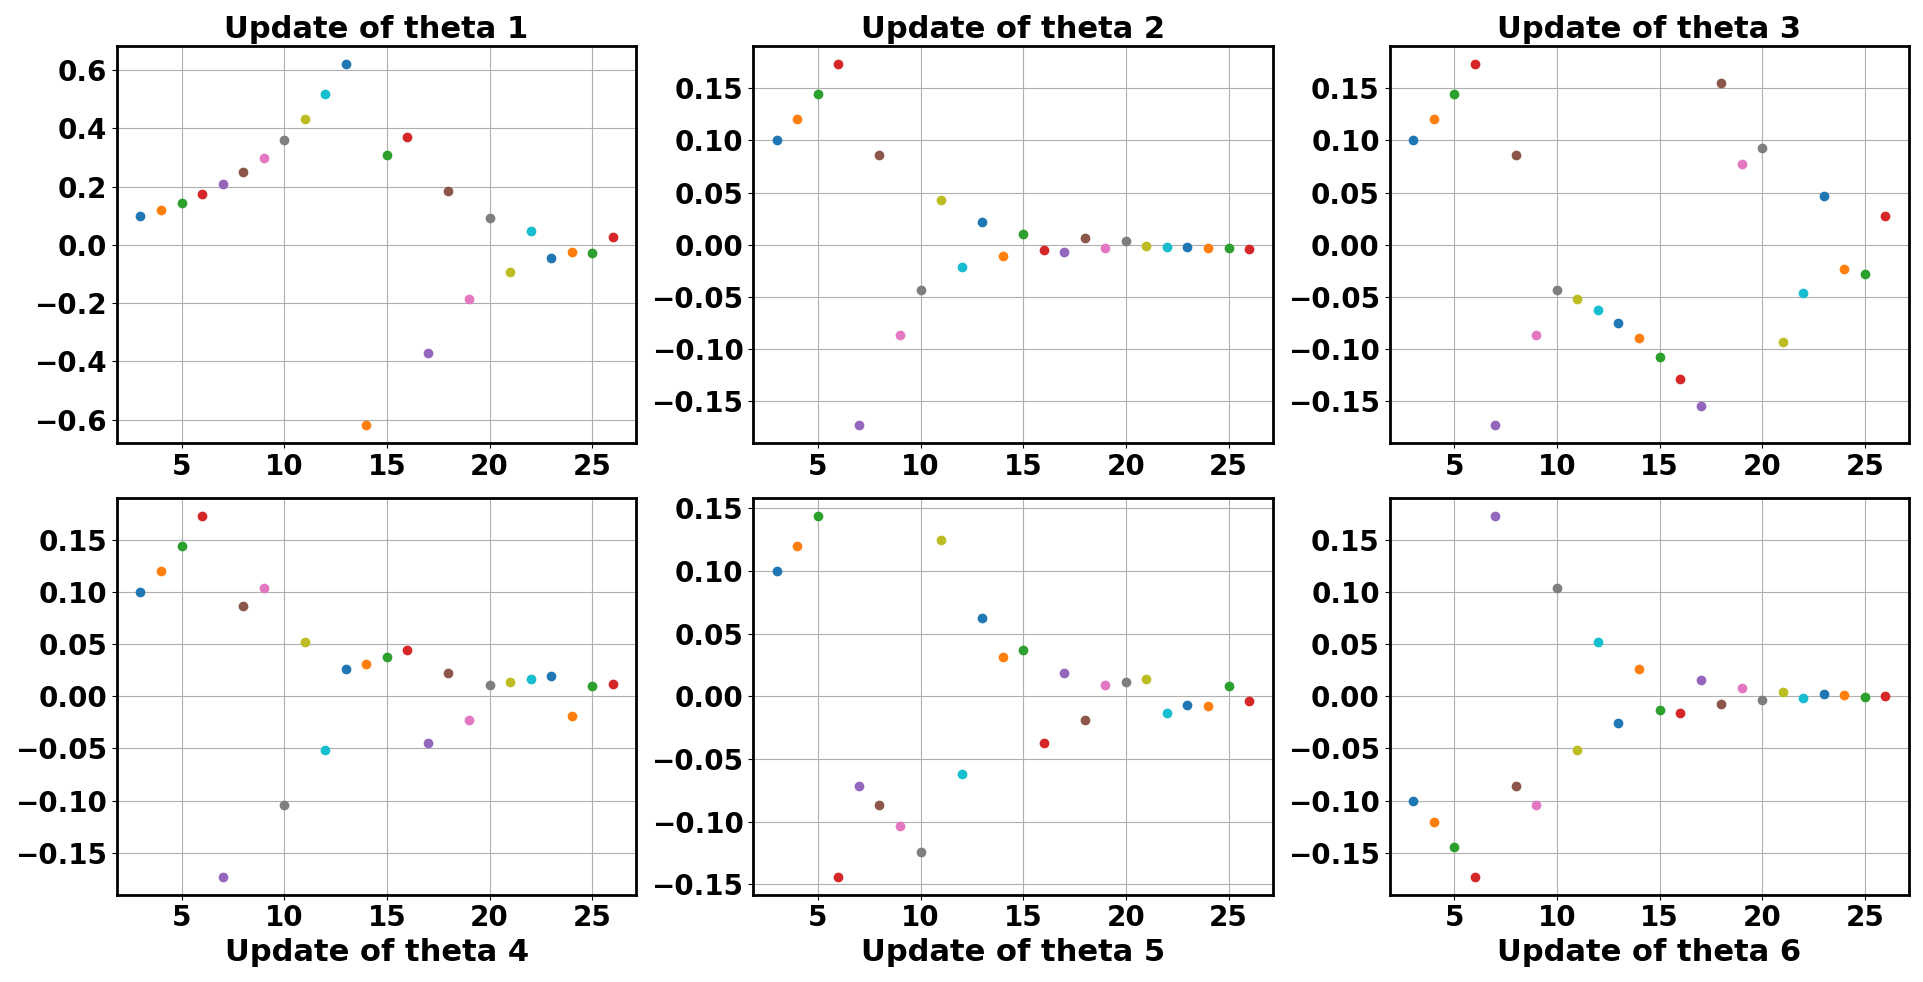
\includegraphics[width=1.0\textwidth]{15l.png}
	\caption{}
	
\end{figure}


\begin{figure}[h!]\label{fig:app_multigrad}
	\centering
	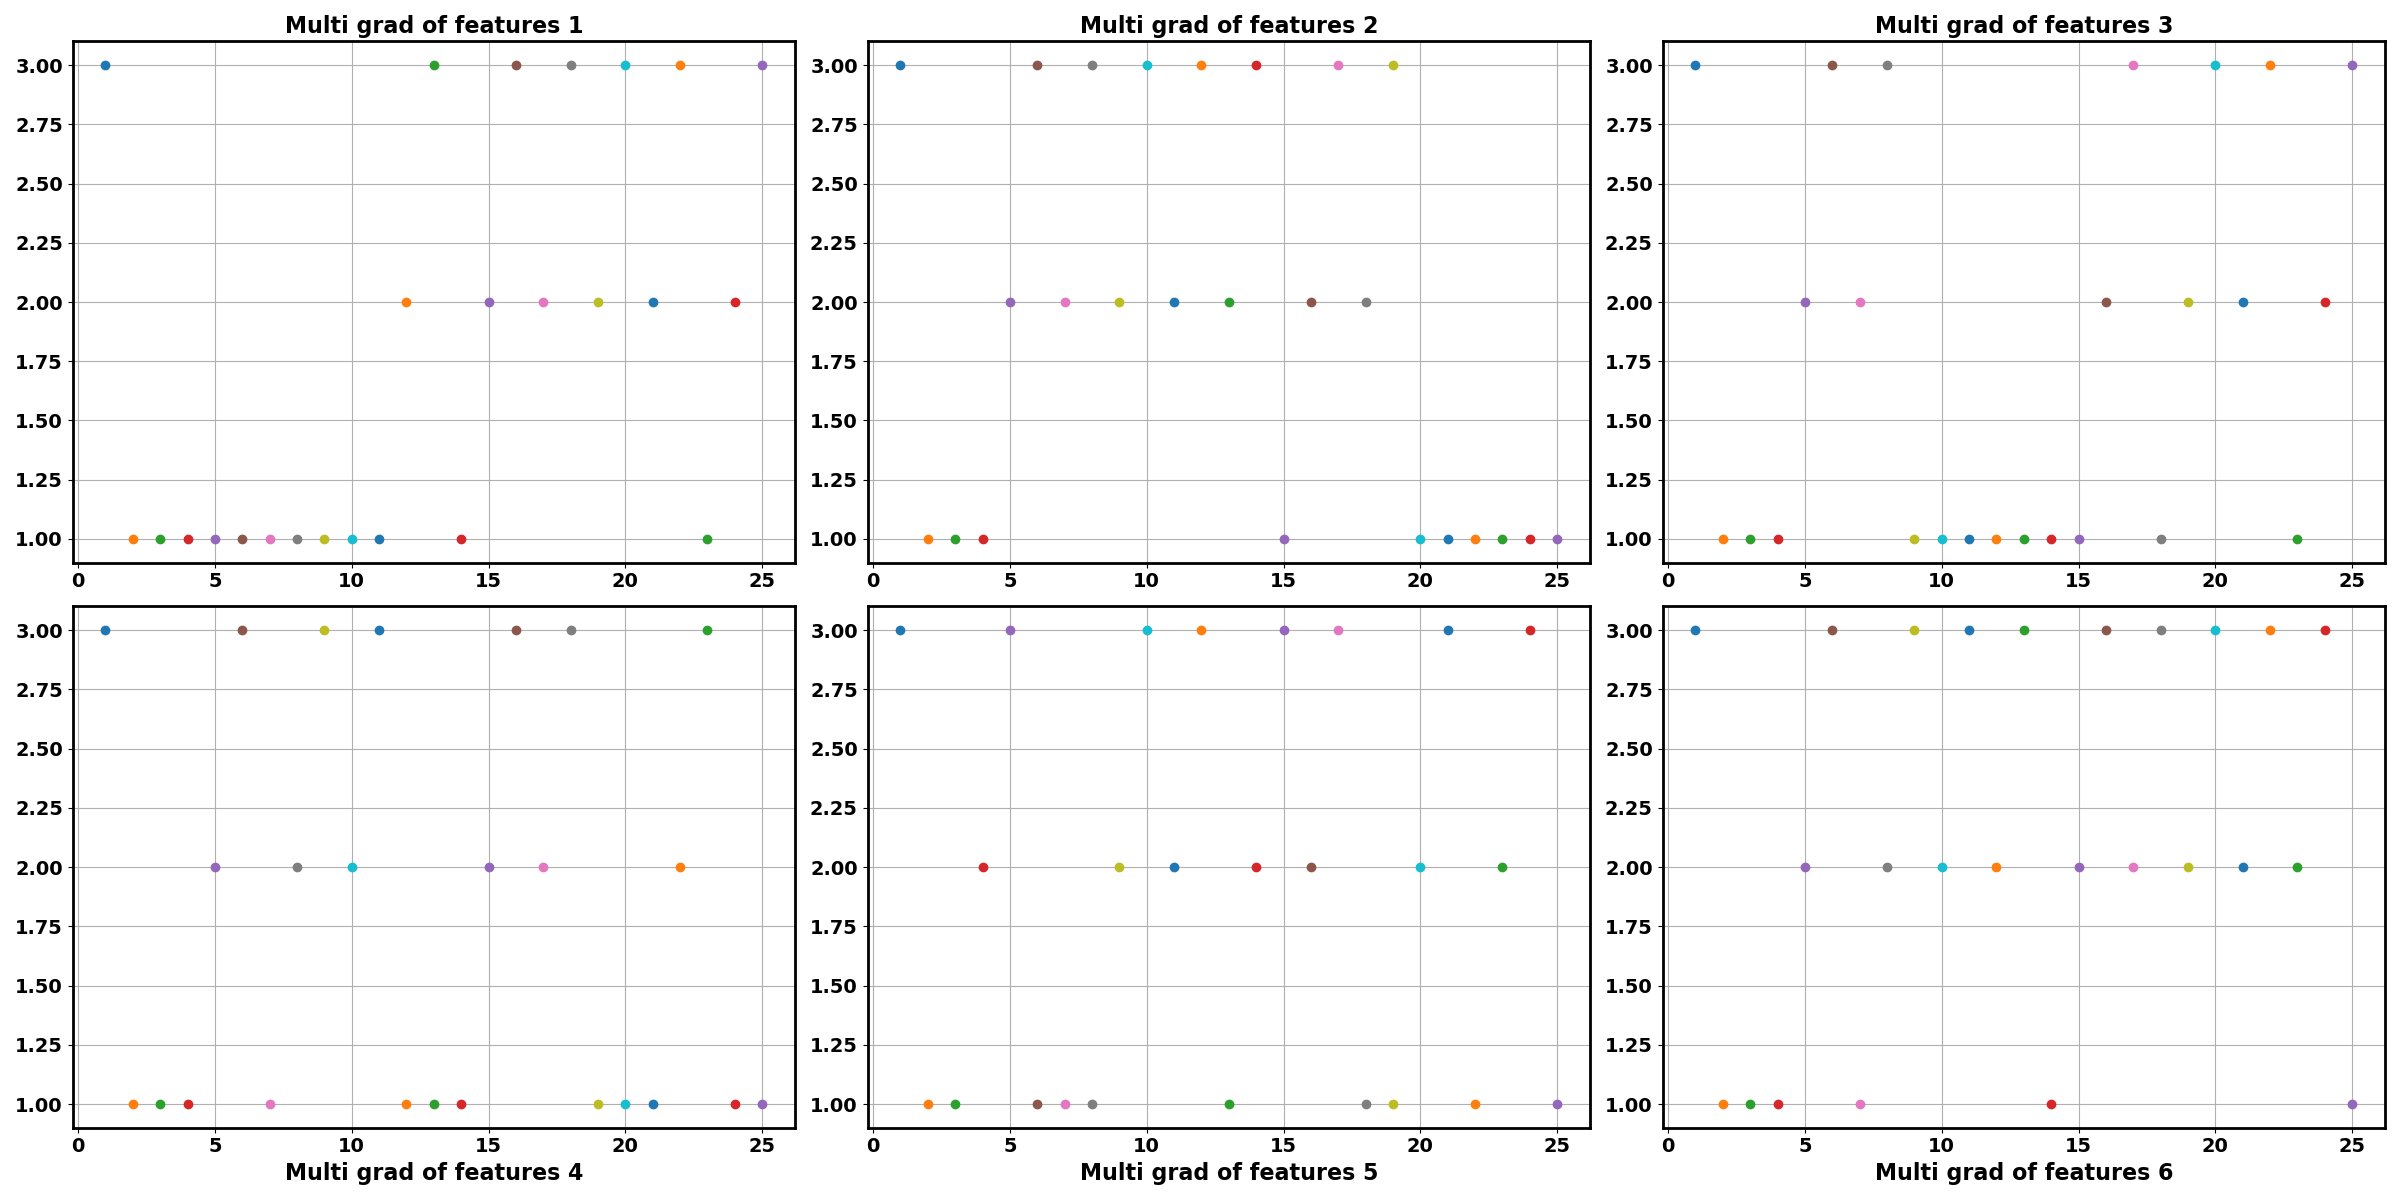
\includegraphics[width=1.0\textwidth]{16l.png}
	\caption{}

\end{figure}












%%% Local Variables: 
%%% mode: latex
%%% TeX-master: "thesis"
%%% End: 
